% This is "sig-alternate.tex" V2.0 May 2012
% This file should be compiled with V2.5 of "sig-alternate.cls" May 2012
%
% This example file demonstrates the use of the 'sig-alternate.cls'
% V2.5 LaTeX2e document class file. It is for those submitting
% articles to ACM Conference Proceedings WHO DO NOT WISH TO
% STRICTLY ADHERE TO THE SIGS (PUBS-BOARD-ENDORSED) STYLE.
% The 'sig-alternate.cls' file will produce a similar-looking,
% albeit, 'tighter' paper resulting in, invariably, fewer pages.
%
% ----------------------------------------------------------------------------------------------------------------
% This .tex file (and associated .cls V2.5) produces:
%       1) The Permission Statement
%       2) The Conference (location) Info information
%       3) The Copyright Line with ACM data
%       4) NO page numbers
%
% as against the acm_proc_article-sp.cls file which
% DOES NOT produce 1) thru' 3) above.
%
% Using 'sig-alternate.cls' you have control, however, from within
% the source .tex file, over both the CopyrightYear
% (defaulted to 200X) and the ACM Copyright Data
% (defaulted to X-XXXXX-XX-X/XX/XX).
% e.g.
% \CopyrightYear{2007} will cause 2007 to appear in the copyright line.
% \crdata{0-12345-67-8/90/12} will cause 0-12345-67-8/90/12 to appear in the copyright line.
%
% ---------------------------------------------------------------------------------------------------------------
% This .tex source is an example which *does* use
% the .bib file (from which the .bbl file % is produced).
% REMEMBER HOWEVER: After having produced the .bbl file,
% and prior to final submission, you *NEED* to 'insert'
% your .bbl file into your source .tex file so as to provide
% ONE 'self-contained' source file.
%
% ================= IF YOU HAVE QUESTIONS =======================
% Questions regarding the SIGS styles, SIGS policies and
% procedures, Conferences etc. should be sent to
% Adrienne Griscti (griscti@acm.org)
%
% Technical questions _only_ to
% Gerald Murray (murray@hq.acm.org)
% ===============================================================
%
% For tracking purposes - this is V2.0 - May 2012



\documentclass{sig-alternate}

\usepackage{times}
\usepackage{amssymb}
\usepackage{epsfig}
\usepackage{subfigure}
\usepackage{graphicx}
\usepackage{amsmath}
\usepackage{tabularx}
\usepackage[ruled,boxed]{algorithm}
\usepackage{algorithmic}
\usepackage{url}
\usepackage{color}
\usepackage{balance}

\sloppy
\newcommand{\LeeWave}{\textsc{LeeWave}}
\newcommand{\MSWave}{\textsc{MsWave}}
\newcommand{\MSWaveH}{{\large \textsc{MsWave}}}
\newcommand{\MSWaveT}{{\LARGE \textsc{MsWave}}}
\newcommand{\argmax}[1]{\underset{#1}{\operatorname{arg}\,\operatorname{max}}\;}
\newcommand{\argmin}[1]{\underset{#1}{\operatorname{arg}\,\operatorname{min}}\;%
}


\newtheorem{example}{Example}
\newtheorem{definition}{Definition}
\newtheorem{theorem}{Theorem}


\renewcommand{\algorithmicrequire}{\textbf{{\small Algorithm:}}} 
\renewcommand{\algorithmicensure}{\textbf{{\small Procedure:}}}
%\pagestyle{empty}

% So Phil can create a pdf without getting a "missing font" error
%\renewcommand{\sum}{\Sigma}
%\renewcommand{\sqrt}[1]{(#1)^{\frac{1}{2}}}

\begin{document}

%
% --- Author Metadata here ---
%\conferenceinfo{WOODSTOCK}{'97 El Paso, Texas USA}
\conferenceinfo{KDD}{'13 Chicago, Illinois USA}
%\CopyrightYear{2007} % Allows default copyright year (20XX) to be over-ridden - IF NEED BE.
%\crdata{0-12345-67-8/90/01}  % Allows default copyright data (0-89791-88-6/97/05) to be over-ridden - IF NEED BE.
% --- End of Author Metadata ---

%\title{A Bandwidth-Efficient Framework for Finding Distributed $k$NN/$k$FN Queries of Multiple Time Series}
\title{\MSWaveT{}: Bandwidth-Efficient Distributed kNN/kFN Search for Multiple Time Series Queries}
%\subtitle{[Extended Abstract]
%\titlenote{A full version of this paper is available as
%\textit{Author's Guide to Preparing ACM SIG Proceedings Using
%\LaTeX$2_\epsilon$\ and BibTeX} at
%\texttt{www.acm.org/eaddress.htm}}}
%
% You need the command \numberofauthors to handle the 'placement
% and alignment' of the authors beneath the title.
%
% For aesthetic reasons, we recommend 'three authors at a time'
% i.e. three 'name/affiliation blocks' be placed beneath the title.
%
% NOTE: You are NOT restricted in how many 'rows' of
% "name/affiliations" may appear. We just ask that you restrict
% the number of 'columns' to three.
%
% Because of the available 'opening page real-estate'
% we ask you to refrain from putting more than six authors
% (two rows with three columns) beneath the article title.
% More than six makes the first-page appear very cluttered indeed.
%
% Use the \alignauthor commands to handle the names
% and affiliations for an 'aesthetic maximum' of six authors.
% Add names, affiliations, addresses for
% the seventh etc. author(s) as the argument for the
% \additionalauthors command.
% These 'additional authors' will be output/set for you
% without further effort on your part as the last section in
% the body of your article BEFORE References or any Appendices.

\numberofauthors{5} %  in this sample file, there are a *total*
% of EIGHT authors. SIX appear on the 'first-page' (for formatting
% reasons) and the remaining two appear in the \additionalauthors section.
%
%\author{
%% You can go ahead and credit any number of authors here,
%% e.g. one 'row of three' or two rows (consisting of one row of three
%% and a second row of one, two or three).
%%
%% The command \alignauthor (no curly braces needed) should
%% precede each author name, affiliation/snail-mail address and
%% e-mail address. Additionally, tag each line of
%% affiliation/address with \affaddr, and tag the
%% e-mail address with \email.
%%
% 1st. author
%\alignauthor
%Ruei-Bin Wang\\
%       \affaddr{Institute for Clarity in Documentation}\\
%       \affaddr{1932 Wallamaloo Lane}\\
%       \affaddr{Wallamaloo, New Zealand}\\
%       \email{trovato@corporation.com}
%% 2nd. author
%\alignauthor
%Yu-Chen Lu\\
%       \affaddr{Institute for Clarity in Documentation}\\
%       \affaddr{P.O. Box 1212}\\
%       \affaddr{Dublin, Ohio 43017-6221}\\
%       \email{webmaster@marysville-ohio.com}
%% 3rd. author
%\alignauthor Mi-Yen Yeh\\
%       \affaddr{Institute of Information Science}\\
%       \affaddr{Academia Sinica}\\
%       \affaddr{Taipei, Taiwan}\\
%       \email{miyen@iis.sinica.edu.tw}
%\and  % use '\and' if you need 'another row' of author names
%% 4th. author
%\alignauthor Shou-De Lin\\
%       \affaddr{Dept. of Computer Science and Information Engineering}\\
%       \affaddr{National Taiwan University}\\
%       \affaddr{Taipei, Taiwan}\\
%       \email{sdlin@csie.ntu.edu.tw}
%% 5th. author
%\alignauthor Phillip Gibbons\\
%       \affaddr{Intel Research}\\
%       \affaddr{ }\\
%       \affaddr{ }\\
%       \email{phillip.b.gibbons@intel.com}
%}
%% There's nothing stopping you putting the seventh, eighth, etc.
%% author on the opening page (as the 'third row') but we ask,
%% for aesthetic reasons that you place these 'additional authors'
%% in the \additional authors block, viz.
%

\author{
\aufnt Ruei-Bin Wang$^{\dagger}$\ \ Yu-Chen Lu$^\dagger$\ \ Mi-Yen Yeh$^\ddagger$\ \ Shou-De Lin$^\dagger$\ \ Phillip B. Gibbons$^\S$\\\\
\affaddr{ $^\dagger$Department of Computer Science and Information Engineering, National Taiwan University, Taiwan}\\ 
\affaddr{ $^\ddagger$Institute of Information Science, Academia Sinica, Taiwan}\\
\affaddr{ $^\S$Intel Labs Pittsburgh, USA}\\\\
\eaddfnt r790822@gmail.com, b98902105@ntu.edu.tw, miyen@iis.sinica.edu.tw, \\  sdlin@csie.ntu.edu.tw, phillip.b.gibbons@intel.com
}

\maketitle
\begin{abstract}

%In the big data era, it is very common to encounter ad hoc snapshot queries that require a fast response from many local machines in which all the data are distributed. In the scenario when the query is more complex such as multiple time series, it is not bandwidth-efficient to send the entire query, comprised of multiple time series, to all the local machines for processing. This paper aims to address this issue. We propose \MSWave{}, a bandwidth-efficient approach to processing distributed $k$NN and $k$FN queries given a reference set of multiple time series. By exploiting Wavelet transformation together with the novel distance bound designs for one-to-many time series, \MSWave{} obtains the exact results of $k$NN and $k$FN queries in a bandwidth-efficient manner. Analytical and empirical studies show that \MSWave{} outperforms the state-of-the-art methods in saving significant bandwidth usage.



In M2M applications, it is very common to encounter the ad hoc snapshot query that requires fast responses from many local machines in which all the data are distributed. In the scenario when the query is more complex, the communication cost for sending it to all the local machines for processing can be very high. This paper aims to address this issue. Given a reference set of multiple and large-size patterns, we propose an approach to identifying its $k$ nearest and farthest neighbors globally across all the local machines. By decomposing the reference patterns into a multi-resolution representation and using novel distance bound designs, our method guarantees the exact results in a communication-efficient manner. Analytical and empirical studies show that our method outperforms the state-of-the-art methods in saving significant bandwidth usage, especially for large numbers of machines and large-sized reference patterns.

\end{abstract}


% A category with the (minimum) three required fields
\category{H.2.8}{Database Management}{Database Applications}[data mining]
%A category including the fourth, optional field follows...
%\category{D.2.8}{Software Engineering}{Metrics}[complexity measures, performance measures]

%\terms{Theory}

\keywords{$k$-nearest/farthest neighbor queries, multiple time-series}

\section{Introduction}\label{sec:intro}

Pattern matching in distributed environments is
generally considered a challenging but important task for applications
relevant to machine-to-machine (M2M) systems. In such
settings where a large amount of local machines are involved in computation and storage, a primary goal is often to minimize the amount of communication
needed to compute the answer.  This paper aims at advancing the
current state-of-the-art on distributed pattern matching from
`single reference pattern' to `multiple reference patterns', and proposes a general framework
to handle both $k$ nearest and farthest neighbor search of the multiple reference pattern set, while
significantly reducing the communication cost, mainly the bandwidth consumption.

Consider a first scenario in which, through sensor data in a specific
area, a scientist detects some unusual and potentially dangerous event
(e.g., the dramatic oscillation of CO2 level), and wants to learn
quickly whether a similar event has happened at other places. To do
so, it is required to use the signal obtained by multiple sensors in
one area to match sensor signals produced in the other areas.  A
second scenario assumes a distributed database of historical sensor
readings such as the past 50 years' temperature information for many
locations.  Researchers might want to specify a set of time series
that they identify with a certain known event (e.g., El Ni\~{n}o,
solar activity, or the increased spread of a pest-borne disease) and
query the distributed database to determine the wheres and whens of
the most similar patterns.  A third scenario assumes that we are
monitoring certain environmental levels at many locations, and we
would like to issue a warning whenever a location's pattern of recent
levels deviates significantly, but perhaps subtly, from the recent
patterns at a set of reference locations, because it might indicate an
abnormal environmental event is happening at that location (e.g.,
hazardous material being improperly transported).

% To accomplish the above task efficiently, one common criteria is minimize the transmission costs between query server and local machines to save bandwidth, energy, and time. have we have a potentially dangerous person to monitor. Say, we want to prevent this person from getting onto any plane. However, what we have are some photos of this person wearing a variety of clothes, while some photos might be clearer than others. An matching  system deployed in security gates of airports would have to take multiple photos as an input, and raise a flag when there is a plausible match. Consider a second scenario, where the photo of every employee in the company are available, and our goal is to design a surveillance system that would issue an warning whenever somebody who does not belong to this company enters any company property. The third scenario in an M2M environment is that assuming we have gathered signals from $M$ different sensors in close-by locations before certain disaster, e.g., tsunami, and would like to design a forecasting system for similar event. In this case, the system has to take the $m$ different time series into account while performing matching. 

Designing a general framework that can handle the above scenarios
requires addressing several challenges. First, the query to be matched
may consist of multiple patterns, in order to provide a more robust
reference set beyond what any one pattern might provide.  For
example, there may be more than one ``signature'' pattern for an event
or more than one nearby sensor monitoring an event.  The multiple patterns
in a single query may be highly correlated, such as when collected by
nearby sensors (1$^{st}$ and 2$^{nd}$ scenarios), or only moderately
correlated, such as when collected from a set of reference locations
(3$^{rd}$ scenario).  Second, the query to be matched is often a
one-time (i.e., snapshot) query, either posed as an ad hoc query
(1$^{st}$ and 2$^{nd}$ scenarios) or as a continuous sequence of
queries such that recent readings determine the next query in the
sequence (3$^{rd}$ scenario).  Third, we need to handle not only
\emph{similarity} (1$^{st}$ and 2$^{nd}$ scenarios) but also \emph{dissimilarity}
(3$^{rd}$ scenario) search.  Fourth, we seek the $k$ most similar (or
$k$ most dissimilar) neighbors from across a potentially large
collection of \emph{distributed} data sources.  Finally, because in
many situations there are bandwidth limitations and concerns of energy
consumption as well as cost during communication, it is usually
critical to design an approach that requires as little communication
between machines as possible. To be more precise, our goal is to reduce
the bandwidth consumption while not missing any $k$ most similar/dissimilar neighbors.

\begin{figure}[tbp]
\centering
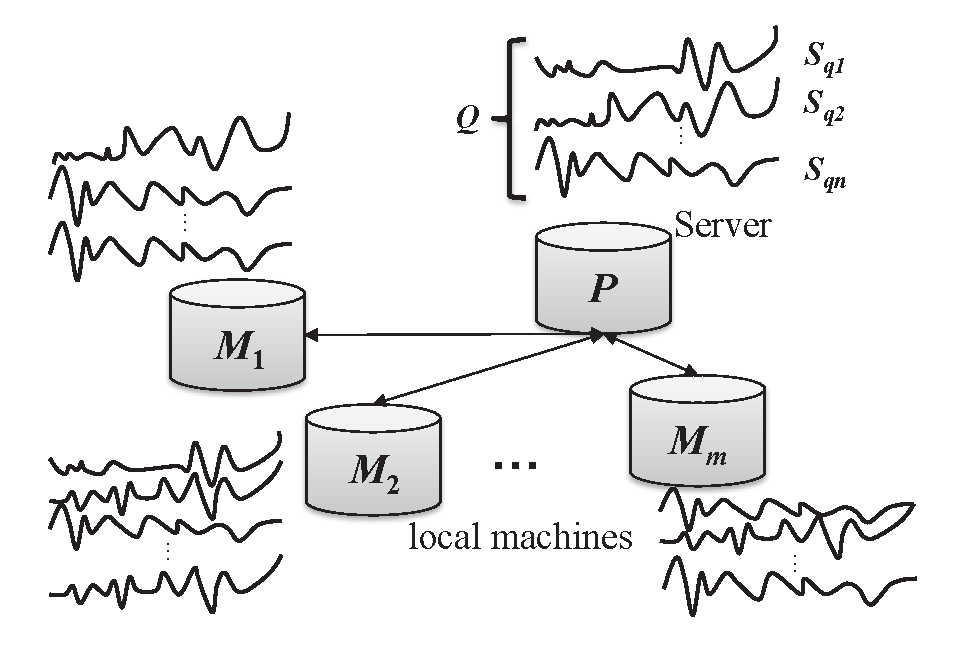
\includegraphics[width=0.6\linewidth]{system-model.eps}
\vspace{-0.1in}
\caption{The system model}
\label{fig:system-model}
\vspace{-0.2in}
\end{figure}

To address the above challenges, we propose a new framework that,
given multiple reference patterns, allows us to find their exact $k$-nearest (most similar) and $k$-farthest (most dissimilar) neighbors, denoted as $k$NN and $k$FN, in a distributed environment where bandwidth is limited. In M2M applications such as the aforementioned three scenarios, a huge amount of measurement readings over a period of time are collected. Therefore the multiple reference patterns to be dealt with in this paper are mainly multiple time series. The system diagram can be seen in Fig.~\ref{fig:system-model}, where there are $m$ distributed machines, each monitoring one or more series of measurement readings, and a server orchestrating
the processing of $k$NN and $k$FN discoveries. Given a set $Q$ of multiple time series patterns as the query at the server, the goal is to find a set of $k$ time series among all $m$ local machines with the highest similarity (or
dissimilarity) to the query.  Our primary cost metric is the total
number of bytes exchanged between the server and the local machines to
answer the query. We do not explicitly model the small cost that may
sometimes be required to assemble the query at the server such as in the 3$^{rd}$
scenario.  Also, while we do not explicitly model response time, our
solutions are highly parallel and fast.

Prior work has considered $k$NN search for the system model in Fig.~\ref{fig:system-model},
but restricted to a single reference pattern (i.e., $|Q|=1$)~\cite{PAP01DPS,Yeh:2008:LLD}.
In a naive solution the server sends the query to each local machine, each local machine computes
the $k$NN to the query from among the locally maintained measurement readings and sends
them back to the server, and finally the server determines the overall $k$NN solution
from among the results received.  This solution, called \textit{Concurrent Processing 
(CP)}~\cite{PAP01DPS}, incurs a high bandwidth cost because 
each of the $m$ machines sends back $k$ results, out of which only $k$ are in the overall
solution.  To address this, Papadopoulos and Manolopoulos~\cite{PAP01DPS} 
proposed the \textit{Probabilistic Processing method (PRP)}, which reduces the amount of data 
required to be transmitted back to the server from the local machines.
To further reduce bandwidth consumption, our earlier work~\cite{Yeh:2008:LLD} proposed
\LeeWave{}, which leverages the multi-resolution property of the Haar wavelet 
transformation of time series. However, none of this prior work considered multiple 
reference patterns or $k$FN search, and straightforward generalizations of \LeeWave{}
produce incorrect results (as we will show in Section~\ref{subsec:limitations}).

Our framework, called \MSWave{}, 
is designed based on the following insights. First, to
handle multiple reference patterns as queries, we propose three distance measurements, 
namely \emph{single-linkage distance}, \emph{average-linkage
distance}, and \emph{complete-linkage distance}, which report the
shortest, average, and largest distances among all the distances of a
candidate time series to each reference pattern in the query set. The above
three distance measures are analogous to the single-link, average-link, and
complete-link clustering models. Second, based on the characteristics
of the Haar wavelet transform, \MSWave{} pre-processes each series of measurement readings by
decomposing it into a multi-resolution representation. Instead of
sending the whole query set $Q$ to the local machines, the server
iteratively sends information on each query in $Q$ in a level-wise manner starting
with the coarsest resolution (fewest bytes sent) and continuing with increasingly finer 
resolutions (more bytes sent).
We further derive and
maintain certain similarity range bounds for each of the three
distance measurements, such that the upper and lower bounds can be incrementally
updated at each iteration/level.  More importantly, we prove that these similarity range
narrow as we move from one wavelet coefficients level to the next,
enabling effective pruning of the candidate time series that reduces bandwidth consumption
without causing any false dismissal.  Although prior work has proposed
wavelet level-wise pruning strategies~\cite{Yeh:2008:LLD, Kashyap:2011:SKS},
we not only generalize it to multiple reference patterns but also further reduce
bandwidth by shifting the similarity bounds calculations from the server
to the local machines.  
%This enables tighter bounds (better pruning) as well as 
%a different communication strategy that saves even more bandwidth.

%We present an analysis demonstrating the significant bandwidth savings from
%shifting the similarity bounds calculations to the local machines.
We conduct extensive experiments using both real and synthetic data. The
results show that our solution significantly outperforms the
competitive approaches in total bandwidth consumption in a variety of
different setups for searching both $k$NN and $k$FN.

Our main contributions can be summarized as follows:
\begin{itemize}
\item
We present \MSWave{}, a general communication-efficient framework to
identify both $k$NN and $k$FN instances given multiple time series reference patterns in
a distributed environment. To our knowledge, this is the
first solution proposed for such purpose.
\item
Methodology-wise, we propose to use average, closest, and
furthest neighbor distance to process multiple query (dis)similarity.
We then take advantage of the multiple-resolution property
of wavelet coefficients, and then for each distance measurement we derive
upper and lower bounds of the similarity between each candidate time series
to the query set. Such bounds can be exploited
to prune candidates for more efficient search without compromising correctness. Moreover,
in further contrast to prior approaches, we propose to shift the
bounds computation from the server to the local machines to further reduce the bandwidth
consumption.
\item
We conduct theoretical analysis and proofs to validate several
of our arguments, including the infeasibility/feasibility of the
existing/proposed approaches, and derive the equation to represent the
bandwidth savings from shifting the bounds computations to the local machines.
Finally, we conduct extensive experiments that demonstrate \MSWave{}'s 
significant bandwidth savings.
\end{itemize}


\section{Preliminaries} \label{sec:prelim} 

In this section we first describe the state-of-the-art approach,
\LeeWave{}, for answering distributed $k$NN queries for a
\emph{single} time series. Then we formally define our distributed
\emph{multiple} time series query problem and discuss why the prior
approach is inadequate for dealing with the proposed problem.


\vspace{-0.1in}
\subsection{Distributed $k$NN for Single Time Series}\label{subsec:single}

The conventional $k$NN (or $k$FN) search for a single reference time
series aims at finding $k$ time series of the smallest (largest)
distance to a given reference time series. In this paper, we will
focus on the Euclidean distance: Given two time series
$\Sref$ and $S_x$ of length $T$, $Dst(\Sref,S_x)$ is defined to be
the squared sum of the Euclidean distance between them.  Namely,
{\small
\begin{equation}\label{eq:squareED} 
Dst(\Sref,S_x)=\sum_{i=1}^{T}{(\Sref[i]-S_x[i])^2},
\end{equation}
}
\noindent\hspace{-0.1in}
where $\Sref[i]$ and $S_x[i]$ are the values of $\Sref$ and $S_x$,
respectively, at timestamp $i$.

To deal with time series matching problems, Wavelet transformation,
especially the Haar Wavelet~\cite{HAA05ZUR}, has been applied in a
variety of studies~\cite{Yeh:2008:LLD,Kashyap:2011:SKS,ZHU03EFF}. In
% as~\cite{BUL03SWA,Kashyap:2011:SKS,TEN04RES,Yeh:2008:LLD,ZHU03EFF}. In
Haar wavelet decomposition, each time series is decomposed into
multiple resolutions and can be represented using an error tree
structure~\cite{MAT98WAV}, as shown in
Fig.~\ref{fig:error-tree}(a). Note that only the non-leaf node
coefficients are retained. The notation $n_{(l,p)}^{(u)}$ shown
in Fig.~\ref{fig:error-tree}(b) is used to represent the coefficient
at level $l$ having offset $p$ of time series $S_u$.

\begin{figure}[t!]
%\vspace{1.75in}
%%\special{psfile=error-tree.eps hscale=32 vscale=32 hoffset=-15 voffset=-150}
%\special{psfile=error-tree.eps hscale=40 vscale=40 hoffset=-20 voffset=-200}
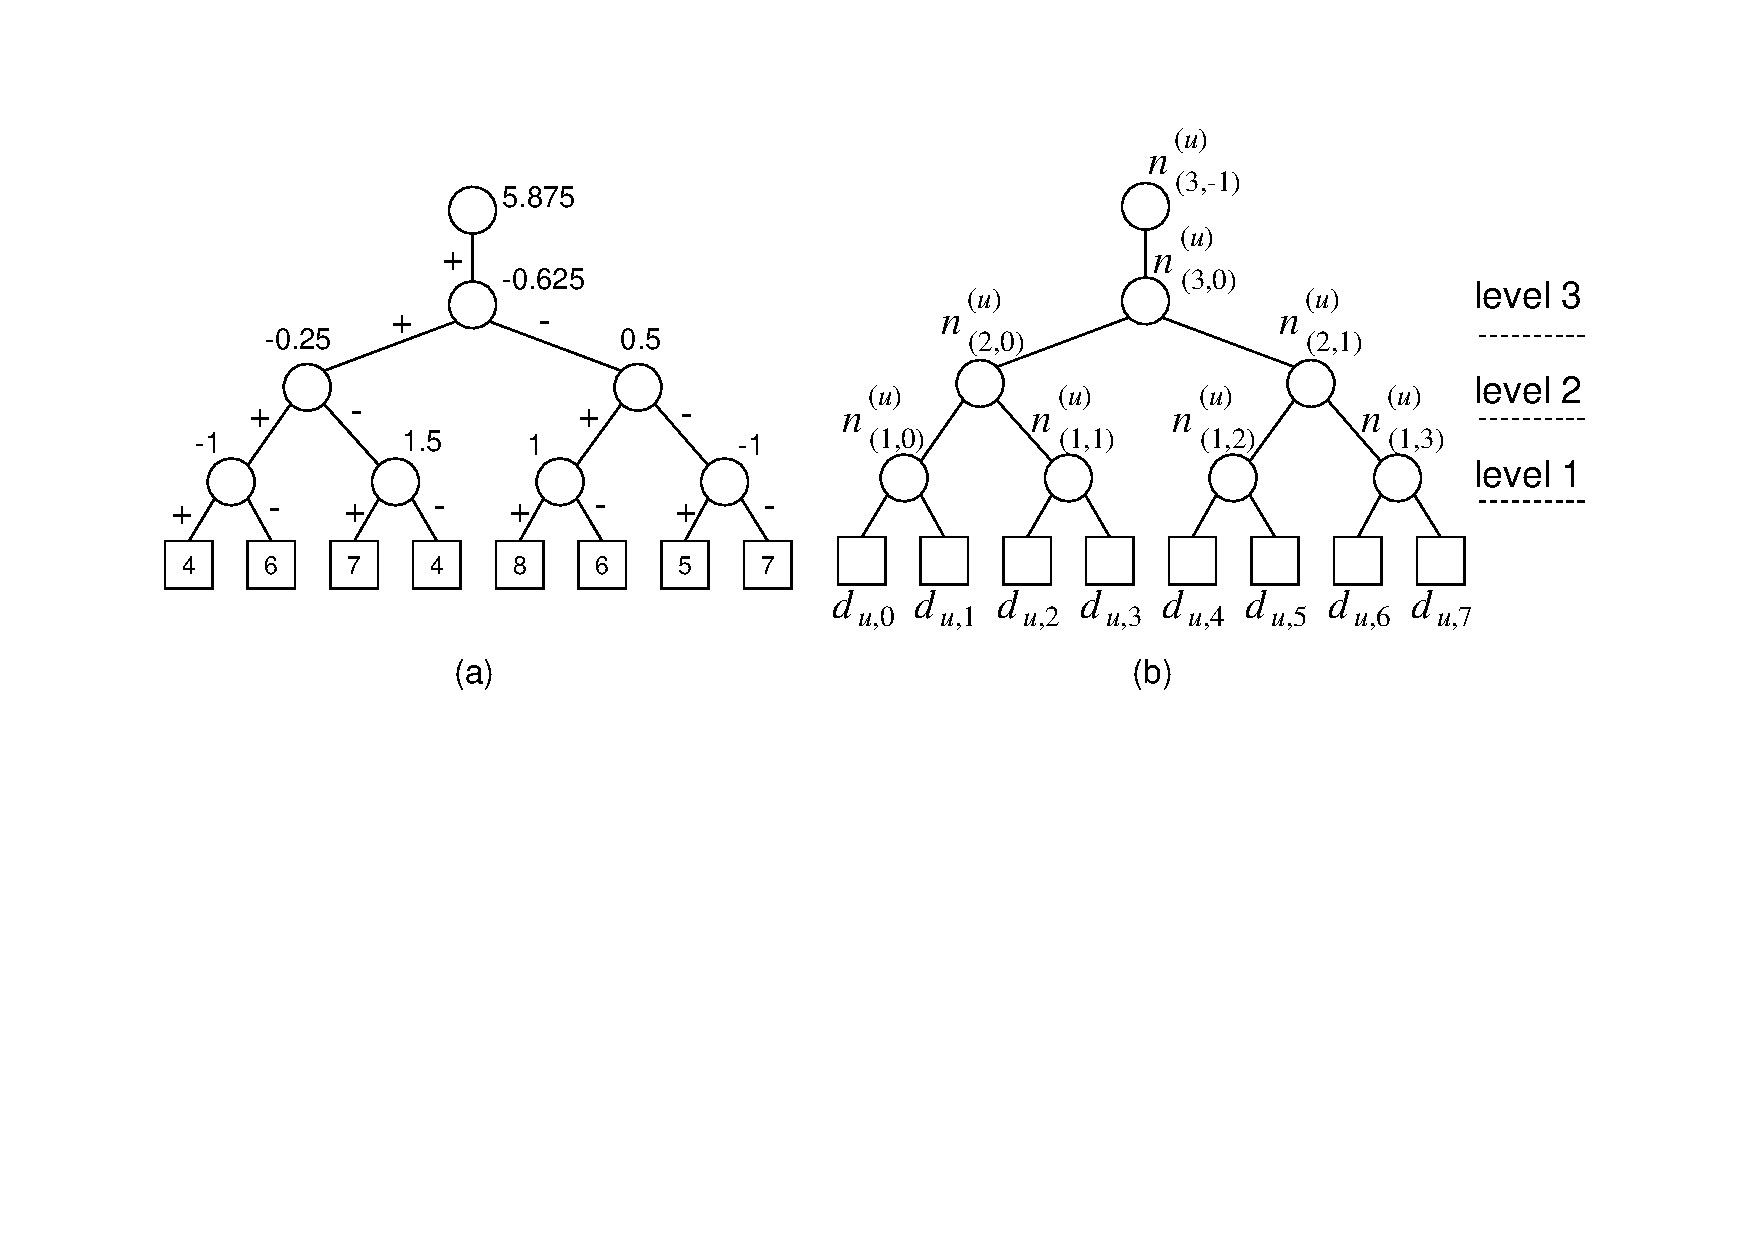
\includegraphics[width=\linewidth]{error-tree.pdf}
\vspace{-0.2in}
\caption{(a) Error tree for a time series \{4,6,7,4,8,6,5,7\}
(b) Error tree notation}
\label{fig:error-tree}
\end{figure}

Given wavelet coefficients of two time series, $Dst(\Sref,S_x)$
can be calculated directly from the coefficients themselves, in a top-down
level-wise manner as suggested in \LeeWave{}~\cite{Yeh:2008:LLD}: 
{\small
\begin{eqnarray}
\lefteqn{Dst(\Sref,S_{x}) = \sum_{l=1}^{L}Dst^{l}(\Sref,S_{x})} \notag \\
& = & accDst^{\ell }(\Sref,S_{x})+\sum_{l=1}^{\ell-1}Dst^{l}(\Sref,S_{x}),
 \label{eq:truedistance} 
\end{eqnarray}
\noindent
where
\begin{equation*}
Dst^{l}(\Sref,S_x)= 2^{l} \times \sum_{p}[n_{(l,p)}^{(\supref)}-n_{(l,p)}^{(x)}]^{2},
\end{equation*}\vspace{-0.1in}
\begin{equation*}
accDst^{\ell}(\Sref,S_x)=\sum_{l =\ell}^{L}Dst^{l }(\Sref,S_x),
\end{equation*}}
\noindent\hspace{-0.1in}
$\ell$ represents the current level, and $L$ is the height of the error tree.

In \LeeWave{}, instead of simultaneously distributing all the relevant
coefficients of the reference series $\Sref$ to all the local machines,
the server only sends the coefficients one level at a time, starting
from the top (the coarsest) level.\footnote{\label{fnt:T}Note
that when the length of a time series is not a power of 2, the
corresponding wavelet coefficients can be represented with multiple
error trees of different heights because any integer value can always
be represented as the summation of distinct powers of two. In such
cases, we still send coefficients from different
sub-trees in a level-wise manner.} Each local machine responds with the
level distance $Dst^{l}(\Sref,S_x)$ for its time series $S_x$ (each machine has
just one time series). Using
such information, the server can determine the similarity range (i.e.,
upper/lower bounds) of each local time series to the reference series:
{\small
\begin{eqnarray}\label{eq:upper-bound}
\lefteqn{accDst^{\ell }(\Sref,S_{x}) \leq Dst(\Sref,S_{x}) \leq} \notag\\
&& accDst^{\ell }(\Sref,S_{x})+\sum_{l=1}^{\ell-1}
  \sum_{p}([n_{(l,p)}^{(\supref)}]^{2}+[n_{(l,p)}^{(x)}]^{2}) \times 2^{l} \notag \\
&& +\ 2 \times \sqrt{\sum_{l=1}^{\ell-1}\sum_{p}[n_{(l,p)}^{(\supref)}\times
  2^{l}]^{2}\times \sum_{l=1}^{\ell-1}\sum_{p}[n_{(l,p)}^{(x)}]^{2}}. 
\end{eqnarray}}

\noindent
Based on these bounds, the server progressively (level-wise) informs
each local machine as to whether its time series is still a candidate for
$k$NN, and if not, the machine drops out of the computation.

Note that the server can compute the lower and upper bounds in
Eq.~(\ref{eq:upper-bound}) from its $n_{(l,p)}^{(\supref)}$ terms and three
summation terms provided by a local machine.  This saves considerable
bandwidth compared to the local machine sending its complete time series.
Also, our earlier work~\cite{Yeh:2008:LLD} proved that the derived upper
bound is non-increasing and the lower bound is non-decreasing when
moving from one level to the next. These increasingly tightened
similarity ranges enable effective pruning of candidates without any
false dismissals.

\vspace{-0.1in}
\subsection{Defining Distributed $k$NN/$k$FN Search for Multiple Time Series}

Before discussing the limitations of the above framework, we first
formulate the distributed $k$NN and $k$FN search problem for multiple
time series.

Let $Q=\{S_{q1},\ldots,S_{qn}\}$ be a set of
$n$ reference time series of length $T$. To match a candidate time
series to the given set of multiple time series, we propose the
following three linkage distances.
\begin{definition} \label{def:3distances}
The \emph{single-link}, \emph{average-link}, and \emph{complete-link}
distances of a time series $S_x$ to a reference set
$Q=\{S_{q1},\ldots,S_{qn}\}$ are defined as:
{\small
\begin{eqnarray*}
d_{sin}(Q, S_x) & = & \min_{1\leq i \leq n}Dst(S_{qi},S_x), \\
d_{avg}(Q, S_x) & = & \sum_{i=1}^{n} Dst(S_{qi},S_x)/n, \text{ and}\\
d_{com}(Q, S_x) & = & \max_{1\leq i \leq n}Dst(S_{qi},S_x). 
\hspace{0.5in}
\end{eqnarray*}}
\end{definition}

These definitions are intended to be analogous to the single-link, average-link, and
complete-link distances used in clustering.  Intuitively, a time
series $S_x$ is considered close to a group of time series $Q$ if either
there exists one time series in $Q$ that is very similar to $S_x$
(i.e., $d_{sin}$), or most of the time series in $Q$ are close
enough to $S_x$ to make their average similar to $S_x$ (i.e., $d_{avg}$), 
or the most dissimilar time series in $Q$ is
still similar to $S_x$ (i.e., $d_{com}$).

With Definition~\ref{def:3distances}, we can now define the distributed $k$NN and
$k$FN search problem for multiple time series queries, referring to Fig.~\ref{fig:system-model}.

\begin{definition}
Given a server $P$ with a reference time series set
$Q=\{S_{q1},\ldots,S_{qn}\}$, each of length $T$, and a set of
distributed local machines $M_1,\ldots,M_m$, each with one or more
time series of length $T$, a \emph{distributed $k$NN ($k$FN) search
for query $Q$} is to find the exact $k$ time series among all the
machines that have the smallest (largest, respectively) linkage
distance, either single-link, average-link, or complete-link as
predefined by the user.  \hfill
\end{definition}

\vspace{-0.1in}
\subsection{Limitations of the Existing Framework}
\label{subsec:limitations}

One immediate question is whether the \LeeWave{} framework from
Section~\ref{subsec:single} can be exploited directly to handle the
multiple time series case.  A simple idea would be to use \LeeWave{}
independently for each of the time series in $Q$, and then try to use
these answers to re-construct the overall $k$NN according to
$d_{sin}$, $d_{avg}$, or $d_{com}$.  We call this framework
\LeeWave-M{}. Unfortunately, considering the 6 cases (3 linkage distance measurements for 
2 kinds of queries), \LeeWave-M{} can guarantee correct
solutions for only 2 of the 6, namely, for $d_{sin}$ in $k$NN and
$d_{com}$ in $k$FN.  To see this, consider the following simple counterexample
for $1$NN search.
\begin{example}
Suppose we have a two length-1 reference time series $S_{q1}$ = \{2\},
$S_{q2}$ = \{-2\}, and candidate time series $S_1$ = \{0\},
$S_2$=\{3\}, and $S_3$=\{-3\} stored in local machine $M_1$ and
candidate time series $S_4$=\{4\} and $S_5$=\{5\} stored in local
machine $M_2$. For $M_1$, $S_2$ gets returned for $S_{q1}$ and $S_3$
for $S_{q2}$; while for $M_2$, $S_4$ gets returned for both reference
series. Considering both machines, $S_2$ is the $1$NN for $S_{q1}$ and
$S_3$ is the $1$NN for $S_{q2}$.  However, the true $1$NN results
under $d_{avg}(Q, S_x)$ and $d_{com}(Q, S_x)$ are both $S_1$, which
was not even selected to be returned to the server.
\end{example}

Similarly, we can find counterexamples for $k$FN under $d_{sin}$ and $d_{avg}$.

Besides the limitation of being able to solve only 2 out of the 6
cases, directly apply \LeeWave-M{} cannot be considered a
bandwidth-efficient approach because each reference series in $Q$ is
processed independently.

The third limitation of \LeeWave{} lies in its server-oriented
computation strategy.  Most of the bounds are calculated on the server
machine based on sum terms sent by the local machines; for the multiple
time series scenario, this strategy wastes bandwidth.

In this paper, we introduce the \MSWave{} framework to deal with the
above limitations.

%In the following, we will introduce how our \MSWave\/ approach solve these challenges. Essentially, the server disseminates the reference time series set in a level-wise manner similar to that in \LeeWave\/. To guarantee no false dismissal when searching for $k$ nearest neighbors to the reference set with only partial information, we show the new bounding computation for the similarity ranges of the three linkage distances of a time series to the reference set. Furthermore, as the reference time series we deal with in \MSWave\/ is multiple, we shift the role of computing the similarity range for each reference-set/candidate-series pair from the server to the local machines. In this way, we can save another significant bandwidth usage compared to the original \LeeWave\/ scheme. Finally, we will show that the same similarity ranges for $k$NN queires can also be used to find the $k$ furthest neighbors.
   





\section{\MSWaveH{} Algorithm and Analysis}
\label{sec:framework}

In \MSWave{}, we also leverage the multi-resolution property of the
Haar wavelet decomposition of time series. The server $P$ distributes
the reference time series set $Q=\{S_{q1},\ldots,S_{qn}\}$ in a
level-wise manner. That is, $P$ sends the coefficients of each $S_{qi}
\in Q$ to the local machines, one level at a time starting from the
highest level $L$.  At each level, we further prune the candidates,
until the final $k$ answers are found.  While similar to \LeeWave{} at
this high level, \MSWave{} must overcome the limitations outlined in
the prior section.  To do this, first we derive new formulas for
computing the similarity ranges of the three linkage distances between
the reference set and a candidate time series
(Section~\ref{subsec:newbounds}).  These ranges must be effective at
pruning yet guarantee no false dismissals.  Second, we devise a
correct and bandwidth-efficient protocol for the data exchanges
between the server and the multiple local machines
(Section~\ref{subsec:protocol}).  We present two variants:
\MSWave-S{}, which computes the bounds at the server, and \MSWave-L{},
which computes the bounds at the local machines.  Finally, we provide
an analysis of the bandwidth consumption of both variants,
which demonstrates the effectiveness of \MSWave{} at reducing bandwidth
(Section~\ref{subsec:analysis}).

\subsection{Problem Setup}\label{subsec:probset}
There are a query set $Q={\{q_1,q_2,...,q_T\}}\subset\mathbb{R}^D$ at the server $P$ and a dataset $X_i\subset\mathbb{R}^D$ on each local machine $M_i$.  For each query $q_t$, we want to find its $k_{th}$ nearest neighborhood among these distributed datasets while reducing the transmission cost between $P$ and each $M_i$.

\subsection{Orthogonal Transformation}
\newtheorem{Orthogonal}{\bf Definition}
\begin{Orthogonal}
A matrix $W \in\mathbb{R}^{D\times D}$ is orthogonal if whose columns and rows are orthogonal vectors, i.e.
\[
W^{T}W=WW^{T}=I
\]
where $I$ is the identity matrix.
\end{Orthogonal}

\newtheorem{ProOfOrthogonal}{\bf Property}
\begin{ProOfOrthogonal}
Let $x, y\in\mathbb{R}^{D}$, and $W\in\mathbb{R}^{D\times D}$ be an orthogonal matrix. Then,
\[
Dist(x,y)^2=\sum^D_{d=1}{(x[d]-y[d])^2} \\
=\sum^D_{d=1}{(W_dx-W_dy)^2}=Dist(Wx,Wy)^2
\]
where $W_d$ is the $d_{th}$ row of $W$.
\end{ProOfOrthogonal}

\subsection{Computation of Distance Bounds}\label{subsec:newbounds}

We start from the similarity range of the distance between each
individual reference time series $S_{qi}$ to some candidate
$S_x$. Similar to Eq.~\eqref{eq:upper-bound}, we can derive the upper
bound $UB$ and the lower bound $LB$ of $Dst(S_{qi},S_x)$ as soon as all the
coefficients for $S_{qi}$ from the highest level $L$ to the current level
$\ell$ have been sent to the local machines, as follows:

{\small
\begin{eqnarray}
\lefteqn{LB(qi,x) =  accDst^{\ell}(S_{qi},S_{x}).} \label{eq:single-LB} \\
\lefteqn{UB(qi,x) = accDst^{\ell }(S_{qi},S_{x})} \notag \\
& + & \sum_{l=1}^{\ell-1}
 \sum_{p}([n_{(l,p)}^{(qi)}]^{2}+[n_{(l,p)}^{(x)}]^{2}) \times 2^{l} \notag \\
& + & 2 \times \min\{\sqrt{\sum_{l=1}^{\ell-1}\sum_{p}[n_{(l,p)}^{(qi)}
 \times 2^{l}]^{2} \times \sum_{l=1}^{\ell-1}\sum_{p}[n_{(l,p)}^{(x)}]^{2}},
   \notag \\
&&\sqrt{\sum_{l=1}^{\ell-1}\sum_{p}[n_{(l,p)}^{(x)} \times 2^{l}]^{2} \times 
        \sum_{l=1}^{\ell-1}\sum_{p}[n_{(l,p)}^{(qi)}]^{2}}\}.
 \label{eq:single-UB}
\end{eqnarray}
}

Note that Eq.~\eqref{eq:single-UB} is an enhanced version of the upper
bound compared to that in Eq.~\eqref{eq:upper-bound}. Because the
roles of $S_{qi}$ and $S_x$ are interchangeable in the squared terms
in Eq.~\eqref{eq:upper-bound}, a tighter upper bound is obtained by
choosing the minimum among the two choices.  Our experiments will show
that this subtle change noticeably improves the pruning
performance. This new bound does not violate the non-increasing
property proved in \cite{Yeh:2008:LLD} because the smaller bound from
two non-increasing bounds is chosen here.

Now we can derive the similarity range for each linkage distance
defined in Definition~\ref{def:3distances}. For $d_{avg}(Q, S_x)$, 
the average of $Dst(S_{qi},S_x)$ for all $S_{qi} \in Q$, we note that because the
distance is non-negative, we can simply derive the new bounds as
follows.

{\small
\begin{align}
&LB_{avg}(Q, S_x)=\frac{1}{|Q|}\sum_{i=1}^{|Q|}LB(qi, x) \label{eq:avg_LB}\\
&UB_{avg}(Q, S_x)=\frac{1}{|Q|}\sum_{i=1}^{|Q|}UB(qi, x) \label{eq:avg_UB}
\end{align}
}

\noindent
For $d_{sin}(Q, S_x)$, the two bounds are:
{\small
\begin{align}
&LB_{sin}(Q, S_x) = \min_{1 \leq i \leq |Q|}LB(qi, x) 
\label{eq:sin_LB}\\
&UB_{sin}(Q, S_x) = \min_{1 \leq i \leq |Q|}UB(qi, x) \label{eq:sin_UB}
\end{align}
}

\noindent
Finally, for $d_{com}(Q, S_x)$, the two bounds are:
{\small
\begin{align}
&LB_{com}(Q, S_x) = \max_{1 \leq i \leq |Q|}LB(qi, x) \label{eq:com_LB}\\
&UB_{com}(Q, S_x) = \max_{1 \leq i \leq |Q|}UB(qi, x) \label{eq:com_UB}
\end{align}
}

\begin{figure}[tbp]
\subfigure[The upper and lower bounds for $d_{sin}(Q,S_x)$.] {
\label{fig:dsinbound}
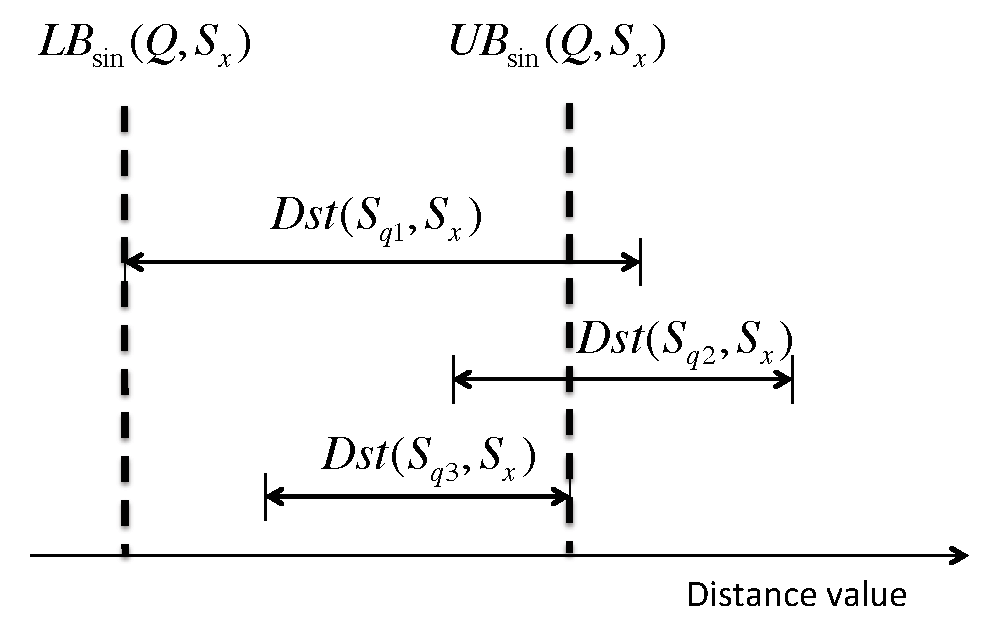
\includegraphics[scale=0.25]{dsinbound.eps}
%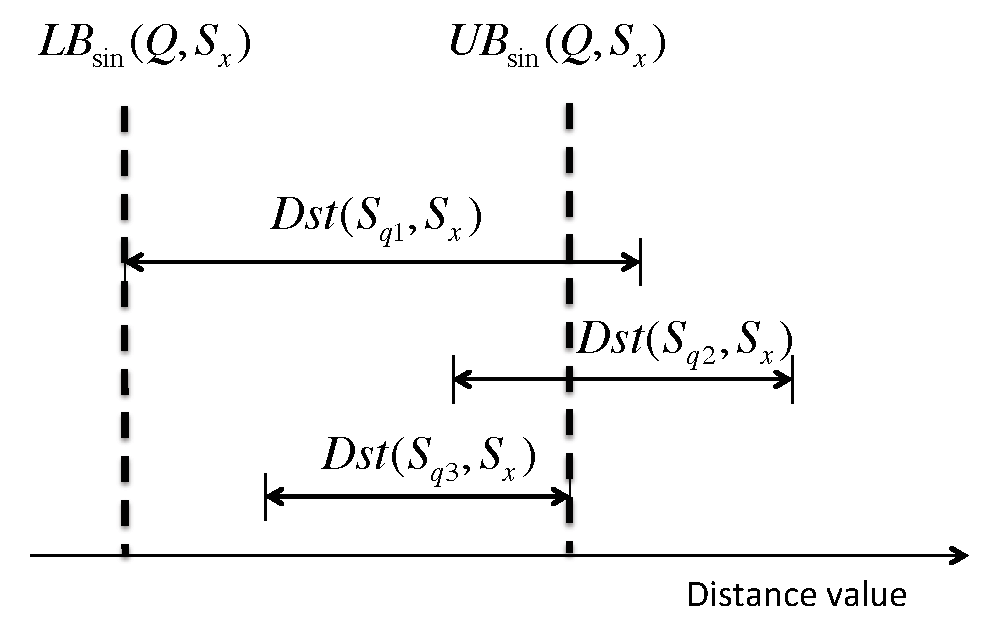
\includegraphics[scale=0.26]{dsinbound.eps}
}
\hspace{0.1cm}
\subfigure[The upper and lower bounds for $d_{com}(Q,S_x)$.] {
\label{fig:dcombound}
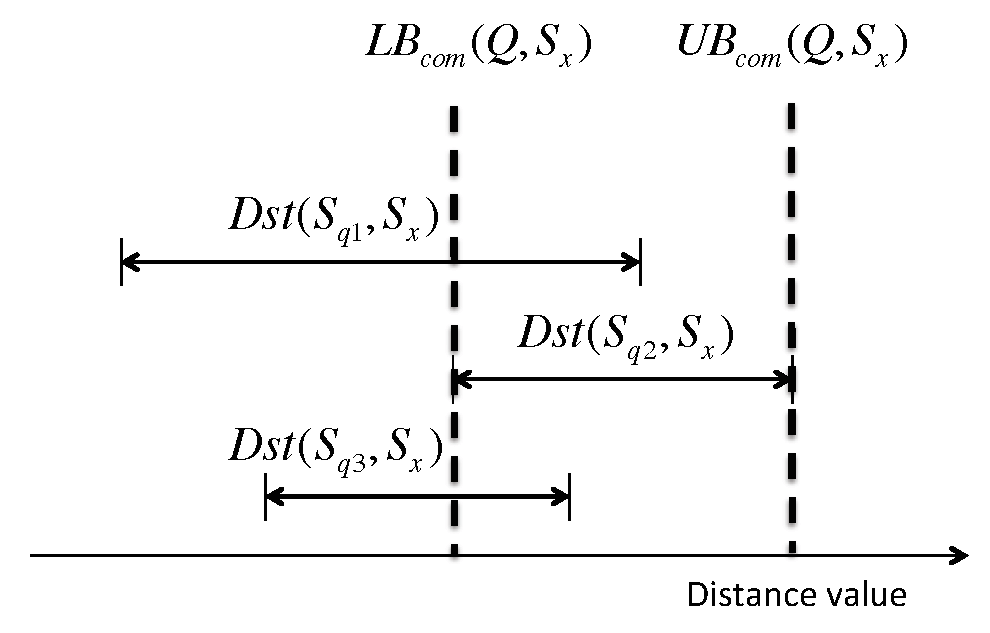
\includegraphics[scale=0.25]{dcombound.eps}
}
\vspace{-0.1in}
\caption{Upper and lower bound computations for different linkage distance measures.}
\label{fig:newbounds}
\vspace{-0.15in}
\end{figure}

Fig.~\ref{fig:dsinbound} illustrates the bounds for $d_{sin}(Q,S_x)$.
As we want to choose the closest distance of
a candidate time series to the reference set $Q$, we can set the lower
(upper) bounds of $d_{sin}(Q,)$ using the smallest ones among all
$LB(qi,x)$ ($UB(qi,x)$, respectively), and for $d_{com}(Q,X)$ using
the largest ones among all $LB(qi,x)$ ($UB(qi,x)$), as shown in
Fig.~\ref{fig:dcombound}.

\begin{figure*}[t!]
\footnotesize
\centering
%\begin{tabular}{|lp{2.95in}|lp{2.95in}|}
\begin{tabular}{|lp{3.2in}|lp{3.2in}|}
\hline
\multicolumn{4}{|p{6in}|}{\textbf{Procedure:} \MSWave-S{} for a $k$NN/$k$FN 
  multiple time series query} \\ 
\multicolumn{4}{|p{6in}|}{\textbf{Input:} $k$, $Q=\{S_{q1},\ldots,S_{qn}\}$, 
  a linkage distance measure (single, average or complete)} \\ 
\multicolumn{4}{|p{6in}|}{\textbf{Output:} The $k$ most similar/dissimilar
  time series to $Q$ according to the designated linkage distance} \\ \hline
\multicolumn{2}{|l|}{\emph{The server $P$:}} & \multicolumn{2}{l|}{\emph{A 
  local machine $M_i$:}} \\
1. & Send coefficients of each $S_{qi} \in Q$ at level $L$ to all  $M$ local 
  machines. & 
2. & For each local candidate time series, $S_x$, compute and return 
  ($Dst^{L}(S_{qi},S_{x})$ $\forall S_{qi} \in Q$, $\sum_{l=1}^{L-1} 
  \sum_{p}[n_{(l,p)}^{(x)}]^{2}$, $\sum_{l=1}^{L-1} 
  \sum_{p}([n_{(l,p)}^{(x)}]^{2}\times 2^l)$, $\sum_{l=1}^{L-1} 
  \sum_{p}([n_{(l,p)}^{(x)}]^{2}\times 2^l)^2$) to $P$. \\ 
3. & Compute the upper and lower bounds based on
  Eq.~\eqref{eq:single-LB}-\eqref{eq:single-UB} for each candidate time series
  to each reference series. Then compute the similarity range for each
  candidate time series to $Q$ according to the designated linkage distance
  based on Eq.~\eqref{eq:avg_LB}-\eqref{eq:com_UB}. Do the first pruning.
  & & \\ 
4. & Repeat steps 5--7 for levels $l=L-1,L-2,\ldots,1$ until \textbf{done}\{
  & & \\ 
5. & Send level coefficients of each $S_{qi} \in Q$ and the ids of any pruned
  candidate series to the appropriate local machines. &
6. & Compute and return a 2-tuple ($Dst^{l}(S_{qi}$, $S_{x})$ $\forall S_{qi}
  \in Q$, $\sum_{p}[n_{(l,p)}^{(x)}]^{2}$) for each local candidate time
  series, $S_x$. \\
7. & Update the upper and lower bounds based on
  Eq.~\eqref{eq:single-LB}-\eqref{eq:single-UB} for each candidate time series
  to each reference series. Then update the bounds of the linkage distance
  based on Eq.~\eqref{eq:avg_LB}-\eqref{eq:com_UB}. Do corresponding pruning
  for $k$NN or $k$FN.  Set \textbf{done} to \textbf{true} if there are
  $k$ candidate time series left. & & \\
8. & \} & & \\
9. & Ask the appropriate machines for the contents
of the final $k$ time series. &
10. & If asked, send back the corresponding full time series contents.\\ \hline
\end{tabular}
\vspace{-0.05in}
\caption{\label{fig:mswave-s}  
Protocol for distributed $k$NN/$k$FN query processing using \MSWave-S{}.}
%\end{figure*}
%
%\begin{figure*}[t]
\vspace{0.15in}
\centering
%\begin{tabular}{|lp{2.95in}|lp{2.95in}|}
\begin{tabular}{|lp{3.2in}|lp{3.2in}|}
\hline
\multicolumn{4}{|p{6in}|}{\textbf{Procedure:} \MSWave-L{} for a $k$NN/$k$FN
  multiple time series query} \\ 
\multicolumn{4}{|p{6in}|}{\textbf{Input:} $k$, $Q=\{S_{q1},\ldots,S_{qn}\}$,
  a linkage distance measure (single, average or complete)} \\ 
\multicolumn{4}{|p{6in}|}{\textbf{Output:} The $k$ most similar/dissimilar time
  series to $Q$ according to the designated linkage distance} \\ \hline
\multicolumn{2}{|l|}{\emph{The server $P$:}} & \multicolumn{2}{l|}{\emph{A
  local machine $M_i$:}} \\
1. & Send level $L$ coefficients,
  $\sum_{l=1}^{L-1} \sum_{p}[n_{(l,p)}^{(qi)}]^2$,
  $\sum_{l=1}^{L-1}\sum_{p}([n_{(l,p)}^{(qi)}]^2 \times 2^{l})$, and
  $\sum_{l=1}^{L-1}\sum_{p}([n_{(l,p)}^{(qi)}]^2 \times 2^{l})^2$
  of each $S_{qi} \in Q$  to all $M$ local machines. & 
2. & For each local candidate time series, $S_x$, compute the individual
  bounds with each reference time series using
  Eq.~\eqref{eq:single-LB}-\eqref{eq:single-UB}. Then compute and return the
  two linkage distances bounds based on
  Eq.~\eqref{eq:avg_LB}-\eqref{eq:com_UB}. \\
3. & Do the first pruning by sorting the upper/lower bounds of each candidate
  series.  & & \\ 
4. & Repeat steps 5--7 for levels $l=L-1,L-2,\ldots,1$ until \textbf{done}\{
  & & \\ 
5. & Send level coefficients of each $S_{qi} \in Q$ and the ids of any pruned
  candidate series to the appropriate local machines. &
6. & Update the corresponding upper/lower bounds based on the computation
  defined in Eq.~\eqref{eq:avg_LB}-\eqref{eq:com_UB} and return the two
  linkage distance bounds for each local candidate time series. \\
7. & Do corresponding pruning for $k$NN or $k$FN according to the updated
  bounds of each candidate series sent back from the local machines.
  Set \textbf{done} to \textbf{true} if there are $k$
  candidate time series left. & & \\
8. & \} & & \\
9. & Ask the appropriate machines for the contents
of the final $k$ time series. &
10. & If asked, send back the corresponding full time series contents.\\ \hline
\end{tabular}
\vspace{-0.05in}
\caption{\label{fig:mswave-l}
Protocol for distributed $k$NN/$k$FN query processing using \MSWave-L{}.}
\end{figure*}

Now we prove the similarity ranges bounded by these lower and upper
bounds will shrink as more levels of coefficients are disseminated to
local machines.

\begin{theorem} \label{theo:avg-bound-shrink}
$UB_{avg}(Q, S_x)$ is non-increasing and $LB_{avg}(Q, S_x)$ is
non-decreasing when the coefficients of $S_{qi} \in Q$ are
disseminated from level $\ell$ to level $\ell-1$
\end{theorem}

\textbf{Proof:} As argued above, it readily follows from
\cite{Yeh:2008:LLD} that Eq.~\eqref{eq:single-LB} is non-decreasing
and Eq.~\eqref{eq:single-UB} is non-increasing. Therefore,
$LB_{avg}(Q, S_x)$ must be non-decreasing and $UB_{avg}(Q, S_x)$ must
be non-increasing as they are each just the average of a set of such
non-decreasing and non-increasing bounds.  \hfill $\blacksquare$

\begin{theorem} \label{theo:sin-bound-shrink}
$UB_{sin}(Q, S_x)$ is non-increasing and $LB_{sin}(Q, S_x)$ is
non-decreasing when the coefficients of $S_{qi} \in Q$ are
disseminated from level $\ell$ to level $\ell-1$
\end{theorem}

\textbf{Proof:} Let $l(\ell)$ and $u(\ell)$ be the reference time
series in $Q$ that have the smallest lower bound and smallest upper
bound of the similarity range to $S_x$ at level $\ell$. That is,

{\small
\begin{eqnarray*}
l(\ell)& = & \arg\min_{1\leq i \leq |Q|}LB(qi,x)|_{\ell}
\hspace{0.3in} \textrm{and}\\
u(\ell)& = & \arg\min_{1\leq i \leq |Q|}UB(qi,x)|_{\ell},
\end{eqnarray*}
}

\noindent
where $|_{\ell}$ represents the corresponding bound values are 
derived at level $\ell$. We have
{\small
\begin{eqnarray*}
\lefteqn{LB_{sin}(Q,S_x)|_\ell = LB(q_{l(\ell)},x)|_\ell 
 \leq LB(q_{l(\ell-1)},x)|_\ell} \\
 &&\leq LB(q_{l(\ell-1)},x)|_{\ell-1} = LB_{sin}(Q,S_x|_{\ell-1}),
\end{eqnarray*}}

\noindent
where the first inequality holds because $l(\ell)$ is the arg min at
level $\ell$ and the second inequality holds because
Eq.~\eqref{eq:single-LB} is non-decreasing.  Thus, $LB_{sin}(Q,S_x)$ is
non-decreasing.

Similarly, because Eq.~\eqref{eq:single-UB} is non-increasing, a symmetric
argument shows that $UB_{sin}(Q,S_x)$ is non-increasing.
\hfill $\blacksquare$

Finally, the symmetry between the bounds for $d_{syn}$ and $d_{com}$
yields the following.
\begin{theorem}
\label{theo:com-bound-shrink}
$UB_{com}(Q, S_x)$ is non-increasing and $LB_{com}(Q, S_x)$ is
non-decreasing when the coefficients of $S_{qi} \in Q$ are
disseminated from level $\ell$ to level $\ell-1$.
\end{theorem}

\vspace{-0.1in}
\subsection{The \MSWave{} Protocol}\label{subsec:protocol}

We are now ready to describe the details of how \MSWave{} processes a
distributed $k$NN or $k$FN multiple time series query in a level-wise
manner and how the server $P$ progressively prunes the candidates. 
We will present two schemes to solve this problem: \MSWave-S{} and \MSWave-L{}. 

\textbf{\MSWave-S{}: Server computes the bounds.}
Fig.~\ref{fig:mswave-s} presents the \MSWave-S{} protocol. At the
initial step, the server $P$ sends the highest level-$L$ coefficients
of each $S_{qi}$ in $Q$ to all $M$ local machines. Each local machine
then extracts wavelet coefficients of the same level for each time
series to be matched.  It then returns the following numbers for each
local candidate time series $S_x$: the level-$L$ distance,
$Dst^{L}(S_{qi}, S_x)$, for $i=1$ to $|Q|$, and three other numbers that
will be used by $P$ to generate the bounds for pruning:
{\small
%\[
$\sum_{l=1}^{L-1}\sum_{p}[n_{(l,p)}^{(x)}]^2$,
$\sum_{l=1}^{L-1}\sum_{p}([n_{(l,p)}^{(x)}]^2 \times 2^{l})$
% \hspace{0.1in}
\textrm{and}
% \hspace{0.1in} 
$\sum_{l=1}^{L-1}\sum_{p}([n_{(l,p)}^{(x)}]^2 \times 2^{l})^2$.
%\]
}
%
%\noindent
After receiving these numbers from each candidate time series, $P$
updates the lower and upper bounds based on Eq.~\eqref{eq:single-LB}
and Eq.~\eqref{eq:single-UB} for each candidate time series.

It then does some initial pruning to remove any candidates that
cannot be among the top $k$ neighbors. To prune candidates for $k$NN
queries, $P$ first sorts the candidate time series in an ascending
order based on the upper bounds.  Any candidate time series whose
similarity lower bound is higher than the upper bound of the $k^{th}$
time series in the sorted list cannot be in the final answer, and thus
is pruned.  As the bound is proved to be monotonically non-increasing
from level to level, we can guarantee that there are no false
dismissals under this pruning strategy. Similarly, for $k$FN query, any
candidate time series whose similarity upper bound is smaller than the
$k^{th}$ largest lower bound cannot be in the final answer. Then, $P$
moves to the next level.

For any given level $l$, $P$ sends the level-$l$ coefficients of each
$S_{qi} \in Q$ and the ids of any pruned time series to the appropriate local
machines.  The local machine returns two level-specific numbers
for each (remaining) candidate time series: $Dst^{l}(S_{qi}, S_x)$ for $i=1$ to
$|Q|$ and $\sum_{p}[n_{(l,p)}^{(x)}]^2$.  $P$ then uses these values to
update the upper/lower bounds, always making them tighter. With the
bounds of each candidate series to each reference time series, $P$
further computes the similarity range under the prespecified linkage distance
of each series to the reference set $Q$ based on
Eq.~\eqref{eq:avg_LB}--\eqref{eq:com_UB}. With increasingly tighter
ranges, $P$ can better prune the candidate list.  The algorithm ends
when there are $k$ candidate time series remaining.

\textbf{\MSWave-L{}: Local machines compute the bounds.}
Note that with \MSWave-S{}, the local machines consume
bandwidth to send back the level distances of each time series to
multiple reference time series, i.e., $Dst^{l}(S_{qi}, S_x)$ for $i=1$
to $|Q|$, which grows linearly with Q. When $|Q|$ becomes large, the
\MSWave-S{} protocol might not be as efficient.

To deal with this issue, we propose another scheme, \MSWave-L{},
which computes the similarity bounds under the linkage distance at the
local machines. By doing so, we need not send the level distances for
each reference time series, but instead only 2 single bound values for
the whole query set, reducing bandwidth.

Fig.~\ref{fig:mswave-l} presents the protocol. In the initial step,
the server $P$ sends to the local machines not only the coefficients
at level $L$, but also three additional numbers for each reference time
series $S_{qi} \in Q$, which will later enable the local machines to
generate the similarity ranges:
{\small
%\[
$\sum_{l=1}^{L-1}\sum_{p}[n_{(l,p)}^{(qi)}]^2$,
$\sum_{l=1}^{L-1}\sum_{p}([n_{(l,p)}^{(qi)}]^2 \times 2^{l})$
% \hspace{0.1in}
\textrm{and}
% \hspace{0.1in} 
$\sum_{l=1}^{L-1}\sum_{p}([n_{(l,p)}^{(qi)}]^2 \times 2^{l})^2$.
%\]
}
%
%\noindent
After receiving these values, the local machines can compute the
similarity bounds of each candidate series to $Q$ based on
Eq.~\eqref{eq:avg_LB}--\eqref{eq:com_UB} according to different linkage
distance measures. Then, each local machine sends back only the two bound
values for each candidate series to the server. With the bounds of
each candidate, the server $P$ can then do corresponding pruning to
tell the local machines which candidates cannot be in the final $k$
results and can be discarded. This procedure proceeds iteratively until the
final results are produced. Note that the pruning strategy is the same
as that done in \MSWave-S{}.


\vspace{-0.1in}
\subsection{Analysis of Bandwidth Consumption}\label{subsec:analysis}

We will now analyze the bandwidth consumption of \MSWave-L{} relative to
\MSWave-S{}. Suppose there are a total of $s$ time series distributed in
$m$ local machines, and $|Q|$ reference time series.
%, and the length of each time series is $T$. For simplicity of exposition, assume $T$ is a power of 2.
%By Haar wavelet decomposition, there will be
%$L=\log_2{T}$ levels of wavelet coefficients for each time series, and
%there are $2^{L-\ell+1}$ number of coefficients at some level $\ell$. 
Let $s_{\ell}$ be the number of candidate time series remaining at
level $\ell$.  We have that the difference in bandwidth between 
\MSWave-S{} and \MSWave-L{} is:
$-3|Q|m + s(4|Q|-2) + \sum_{\ell}{ 2s_{\ell}(|Q|-1) }$, which equals
{\small
\begin{equation}
|Q|( 4s -3m +2\sum_{\ell}{s_{\ell}} ) -2s - 2\sum_{\ell}{s_{\ell}}.
 \label{eq:bandwidthsaved}
\end{equation}
}

\noindent
The term $-3|Q|m$ refers to the three more summation values
sent by $P$ to local machines in step 1 in \MSWave-L{}. The term
$s(4|Q|-2)$ is the bandwidth saved by transmitting only the 2 bounds
for each $\{Q, S_x\}$ instead of all pair-wise reference-candidate
level distances and the related summation values in step 2. The final
summation term describes the bandwidth saved at the following steps
when more and more levels of coefficients are disseminated.

Note that Eq.~\eqref{eq:bandwidthsaved} is always
greater than zero.  Because in general cases $s \geq m$ (otherwise the
data do not have to be distributed to $m$ machines), we have
$|Q|(4s-3m)-2s>(|Q|-2)s \geq 0$, because $|Q|>1$ for multiple
time series, and the final term $2s(|Q|-1)$ is also greater than zero.
Moreover, \MSWave-L{}'s bandwidth savings over \MSWave-S{} increases
linearly with $|Q|$.

%Consequently, the bandwidth consumption for \MSWave-S{} is

%{\footnotesize
%\begin{align}
%&|Q|*M*2 + |Q|*N*4 + N + \notag\\
%&\sum_{\ell}{(|Q|*M_{\ell}*2^{L-\ell+1} + |Q|*N_{\ell}*2+N_{\ell})},
%\label{eq:cost_of_mswave-s}
%\end{align}
%}
%and for \MSWave-L{} is
%{\footnotesize
%\begin{align}
%& |Q|*M*(2+3) + N*(2+1) + \notag\\
%& \sum_{\ell}{(|Q|*M_{\ell}*2^{L-\ell+1} + N_{\ell}*(2+1))},
%\label{eq:cost_of_mswave-l}
%\end{align}
%}
%where $M_{\ell}$ and $N_{\ell}$ is the number of machines having candidate time series and the number of candidate time series left at level $\ell$.

%By subtracting Eq.~\eqref{eq:cost_of_mswave-s} from Eq.~\eqref{eq:cost_of_mswave-l} we have the bandwidth saved by \MSWave-L{} compared to \MSWave-S{} as follows.

\section{Experiments}\label{sec:exp}

The goal for this section is twofold. First, we would like to compare
the bandwidth consumption of \MSWave{} with some baseline and
state-of-the-art approaches. Second, we intend to provide some discussions
on a variety of scenarios and configurations.

\subsection{Data Description and Experiment Setup}\label{subsec:setup}

We use one real data set and one synthetic data set in our experiments. For the real data set,
we choose a public dataset recording the daily average temperature of
300 cities around the world acquired from the temperature data archive
of the University of Dayton. The data from each city is considered as a
time series with 2048 data points. 
For the synthetic data set, we use the same random walk data model used in \cite{Rakthanmanon:2012:SMT}. Each time series is generated by the random walk whose every step size is a normal distributed random number with mean=0 and standard deviation=1. There are 12,500 time series of length 12,500 generated.
After selecting $|Q|$ time series as
the reference set, the candidate time series are chosen from the remaining
time series and are equally distributed to the $m$ machines.

We consider five frameworks: (i) CP, which is the Concurrent
Processing baseline~\cite{PAP01DPS} described in
Section~\ref{sec:intro}, but generalized to $|Q| > 1$ by sending the
whole query set at the beginning; (ii) PRP, which is the Probabilistic
Processing method~\cite{PAP01DPS} mentioned in Section~\ref{sec:intro}, 
but again generalized to $|Q| > 1$ in a straightforward manner;
(iii) \LeeWave-M{}, as discussed in Section~\ref{subsec:limitations};
(iv) \MSWave-S{} (Fig.~\ref{fig:mswave-s}); and 
(v) \MSWave-L{} (Fig.~\ref{fig:mswave-l}).

We compare the total bandwidth cost for these five frameworks in a
distributed environment simulated in MATLAB. We study the influences 
on the bandwidth cost of the size of the reference set $|Q|$, the time series 
length $T$, the number of machines $m$, and the $k$ for $k$NN/$k$FN.
The total bandwidth
cost is the summation of all data transmitted between the server and
other local machines. Note that in this simulation framework,
practical issues such as the overheads of message headers, packet losses,
retransmissions, etc.~were not considered.

There are two strategies we employ to choose the time series that
comprise the instances in a query set $Q$.
For the \emph{analogous reference set}, we choose one time series randomly
and then choose its closest $|Q|$-1 neighbors to form $Q$; thus the queries
in $Q$ are highly similar.
For the \emph{random reference set}), we choose $|Q|$ time series at random;
thus the queries in $Q$ are likely to be dissimilar.

\begin{figure}[tb]
\centering
\subfigure[random reference set] {
\label{fig:1(a)}
%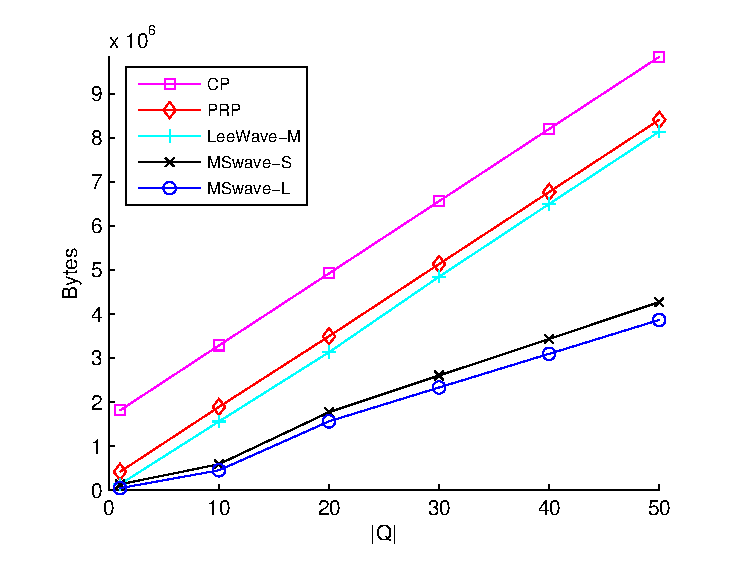
\includegraphics[scale=0.3]{1(a).eps}
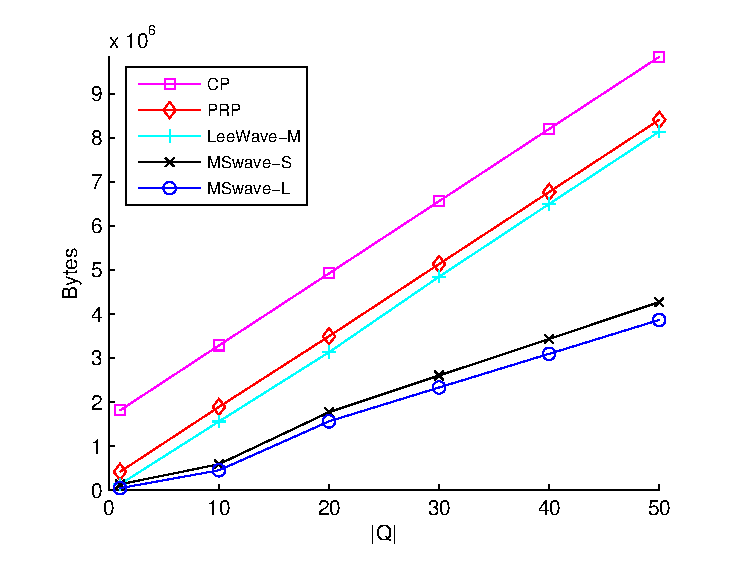
\includegraphics[scale=0.5]{1(a).eps}
}
\subfigure[analogous reference set] {
\label{fig:1(b)}
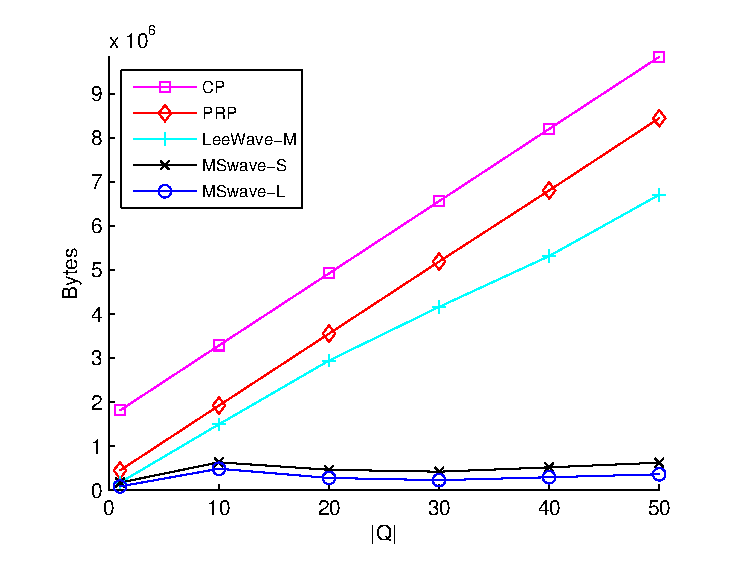
\includegraphics[scale=0.5]{1(b).eps}
}
\vspace{-0.05in}
\caption{\label{fig:1}
Comparison between frameworks given two kinds of query sets, $T$=1024, 
$k$=10, $m$=20, $d_{com}$, and $k$FN}
\vspace{-0.05in}
\end{figure}

\begin{figure*}[t!]
\centering
\subfigure[$k$=10, $|Q|$=10,  $d_{com}$,  $k$FN] {
\label{fig:2(a)}
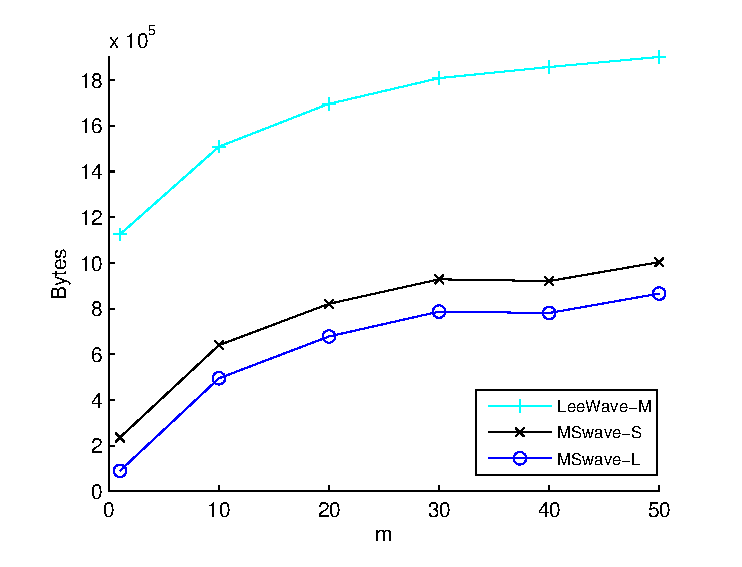
\includegraphics[scale=0.45]{2(a).eps}
}
\hspace{0.1cm}
\subfigure[$k$=10, $|Q|$=10, $d_{sin}$, $k$NN] {
\label{fig:2(b)}
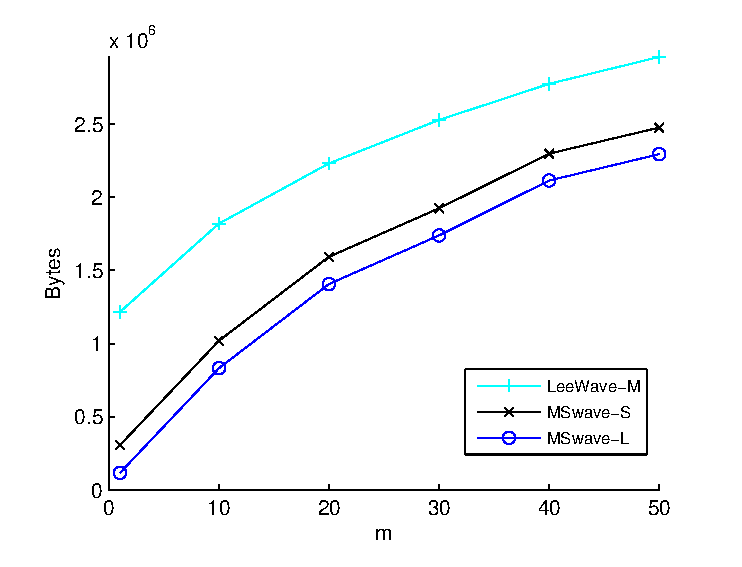
\includegraphics[scale=0.45]{2(b).eps}
}
\hspace{0.1cm}
\subfigure[$k$=10, $m$=20,  $d_{com}$, $k$FN] {
\label{fig:2(c)}
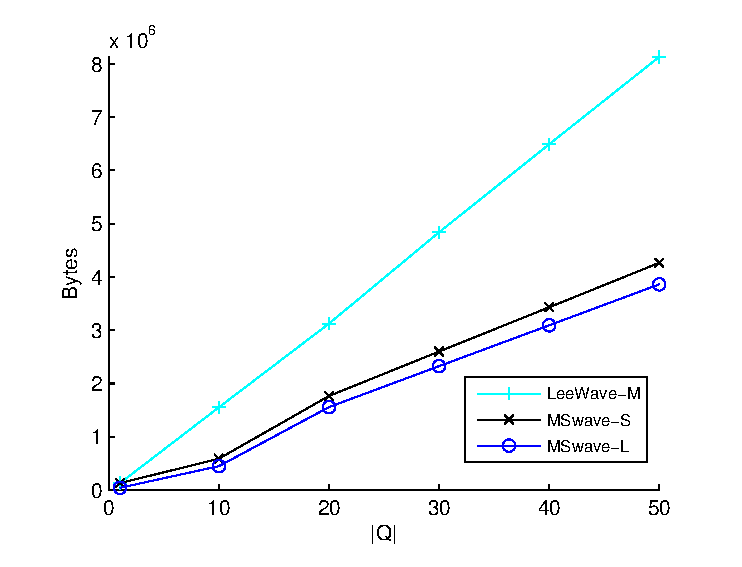
\includegraphics[scale=0.45]{2(c).eps}
}
\hspace{0.1cm}
\subfigure[$k$=10, $m$=20, $d_{sin}$,  $k$NN] {
\label{fig:2(d)}
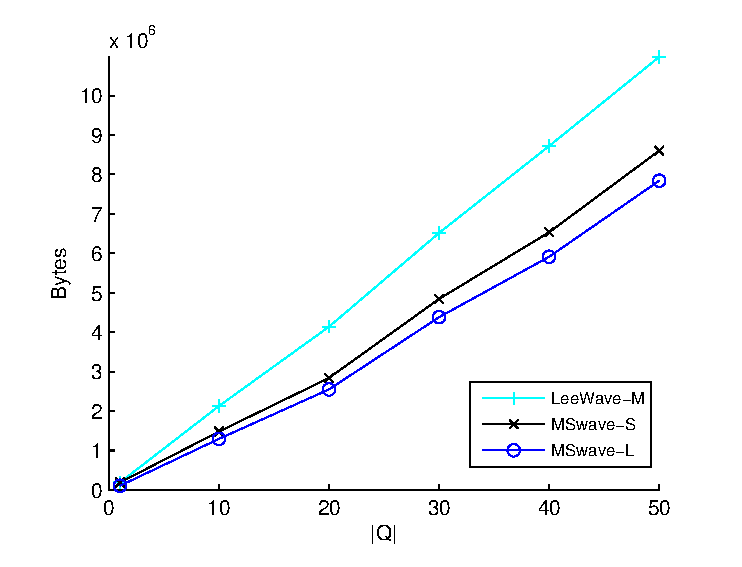
\includegraphics[scale=0.45]{2(d).eps}
}\hspace{0.1cm}
\subfigure[$m$=20, $|Q|$=10, $d_{com}$,  $k$FN] {
\label{fig:2(e)}
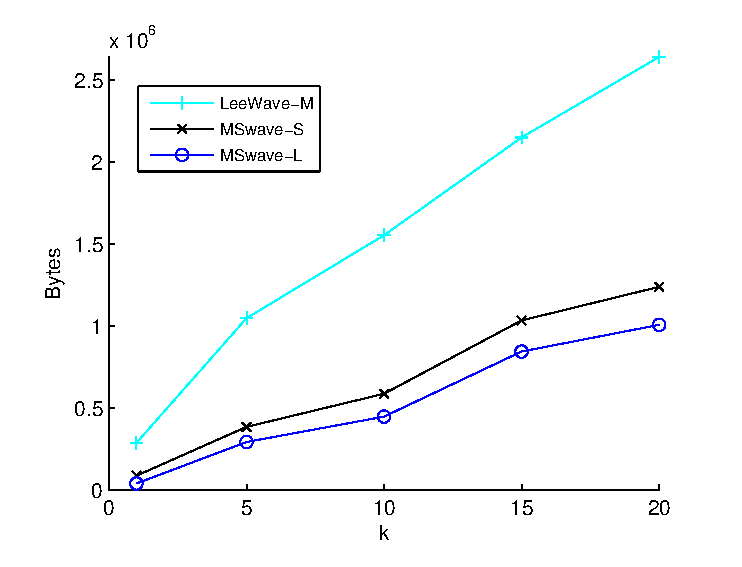
\includegraphics[scale=0.45]{2(e).eps}
}\hspace{0.1cm}
\subfigure[$m$=20, $|Q|$=10,  $d_{sin}$, $k$NN] {
\label{fig:2(f)}
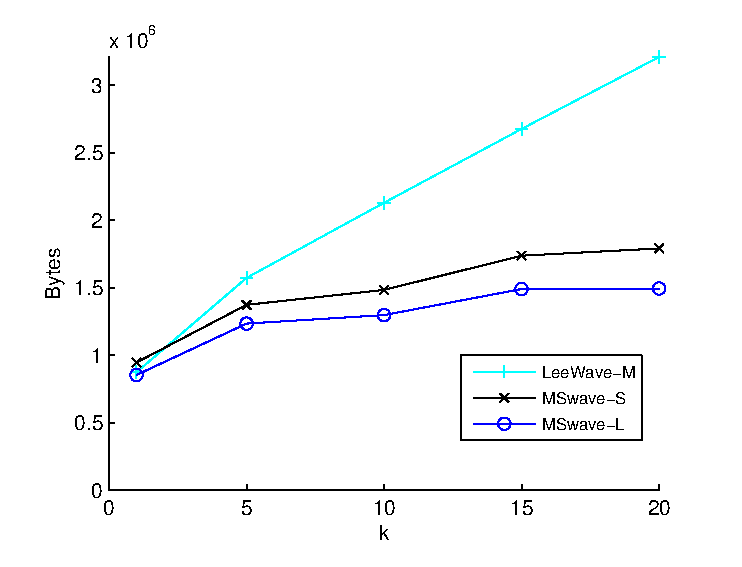
\includegraphics[scale=0.45]{2(f).eps}
}
\vspace{-0.05in}
\caption{Comparison between frameworks given the random reference set, 
$T$=1024.}
\label{fig:2}
\end{figure*}

\subsection{Comparison on Real Data}

\textbf{Comparing all five frameworks.}
Fig.~\ref{fig:1} shows a comparison of the total bandwidth consumption
of all five frameworks, for both the random reference set (Fig.~\ref{fig:1}(a))
and the analogous reference set (Fig.~\ref{fig:1}(b)).
Both plots show that the \MSWave{} frameworks outperform the
other frameworks significantly. We also find the slopes of \MSWave{}
frameworks are
less steep than the slopes of the others, highlighting the benefits of
using Eq.~\eqref{eq:avg_LB}$-$\eqref{eq:com_UB} for pruning. For
analogous reference sets, we even find that the bandwidth costs of the 
\MSWave{} frameworks do not increase significantly when $|Q|$ increases. 
This can be explained as follows. When the reference time series are 
similar, the distance to any one of the reference time series is very 
close to the distance to the whole reference set. This holds regardless of 
whether $d_{avg}$, $d_{sin}$, or $d_{com}$ is chosen. Therefore, in
the early levels of the protocol, we already obtain enough information
to estimate the true distance, which leads to more effective
pruning. On the other hand, for the random reference set, because the
distances to each reference vary a lot, it is generally required to
send many levels of coefficients to be able to accurately estimate the
true distance to determine the $k$NN/$k$FN neighbors, thus consuming
more bandwidth.

\textbf{Comparing \MSWave-L{}, \MSWave-S{} and \LeeWave-M{}.}  Next,
Fig.~\ref{fig:2} highlights the comparison of \MSWave-S{}, \MSWave-L{},
and \LeeWave-M{} in total bandwidth consumption. 
We choose $k$NN for $d_{sin}$ (Fig.~\ref{fig:2(b)}, \ref{fig:2(d)},
\ref{fig:2(f)}) and $k$FN for $d_{com}$ (Fig.~\ref{fig:2(a)},
\ref{fig:2(c)}, \ref{fig:2(e)}) because, as argued in
Section 2.3, these are the only two feasible cases for \LeeWave-M{}.
The figure shows that the performance of \MSWave-L{}
is clearly better than \MSWave-S{}, while both are much better than
\LeeWave-M{} in all configurations.
 
Figs.~\ref{fig:2(a)} and \ref{fig:2(b)} present the results while
varying the number of machines $m$ from 1 to 50. The figures show that
increasing $m$ does not change the performance differences
significantly.  Figs.~\ref{fig:2(c)} and \ref{fig:2(d)} study the
performance impact of the size of reference set $|Q|$, which is varied 
from 1 to 50.  The figures show that the \MSWave-L{}'s bandwidth
savings over \LeeWave-M{} increases as $|Q|$ increases. On
the other hand, while \MSWave-L{}'s bandwidth savings over \MSWave-S{}
also increases as $|Q|$ increases, the increase is less significant.
The savings increases because, the larger the reference
set is, the more values \MSWave-S{} has to send from the local machines to
the server, as analyzed in Section~\ref{subsec:analysis}. Finally,
Figs.~\ref{fig:2(e)} and \ref{fig:2(f)} examine the impact of $k$ on 
the performance, with $k$ varying from 1 to 20.
It is not hard to reason that the difference
between \LeeWave-M{} and \MSWave-L{} in bandwidth consumption
increases as $k$ increases because \LeeWave-M{}'s overhead grows linearly with
$k$. We can also see that the difference between \MSWave-L{} and
\MSWave-S{} increases slightly as $k$ becomes larger. The larger $k$ is,
the fewer candidate series are pruned early, and based on our discussion in
Section~\ref{subsec:analysis}, the gap becomes larger when there are more 
candidate series still remaining.

\textbf{Comparing the upper bounds in Eq.~\eqref{eq:upper-bound} and
Eq.~\eqref{eq:single-UB}.} Table \ref{tbl:bound} compares our new upper
bound in Eq.~\eqref{eq:single-UB} to the upper bound derived in \LeeWave{} 
in Eq.~\eqref{eq:upper-bound}. The
parameters in this experiment are $d_{avg}$ in $k$FN, random reference
set, $T$=1024, $k$=10, $m$=150, and $|Q|$=10. The new bounds
are slightly lower, which makes them better for pruning, although
the improvement is quite small.

\begin{table*}[tb]
\centering
\caption{New bound (Eq.~\eqref{eq:single-UB}) vs old bound (Eq.~\eqref{eq:upper-bound}) , $T$=1024, $k$=10, $m$=150, $|Q|$=10}
\label{tbl:bound}
\vspace*{0.05in}
\begin{tabular}{|l|l|l|l|l|l|l|l|l|l|l|l|}
\hline
step & 1 & 2 & 3 & 4 & 5 & 6 & 7 & 8 & 9 & 10 & 11 \\ \hline
new bound & 150.0 & 150.0 & 148.9 & 137.3 & 53.9 & 32.5 & 24.8 & 19.8 & 15.2 & 11.5 & 8.0 \\ \hline
old bound & 150.0 & 150.0 & 150.0 & 139.1 & 62.4 & 33.7 & 26.0 & 20.3 & 15.6 & 11.5 & 8.0 \\ \hline
\end{tabular}
\vspace{0.1in}
\end{table*}

\begin{figure*}[t]
\centering
\subfigure[Bandwidth consumption under different $|Q|$ and $m$] {
\label{fig:Y3(a)}
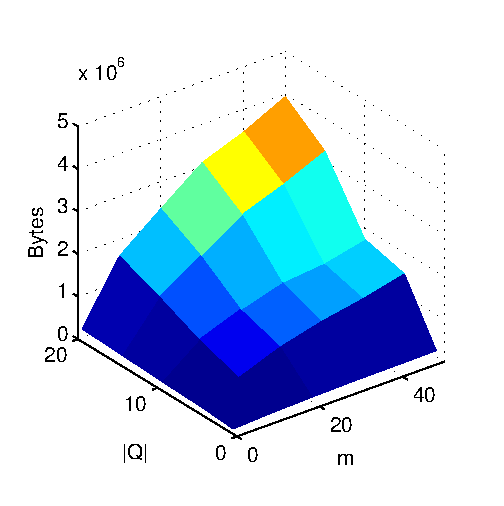
\includegraphics[scale=0.45]{Y3(a).eps}
}
\hspace{0.1cm}
\subfigure[Number of candidate machines in each level, $m$=50] {
\label{fig:Y3(b)}
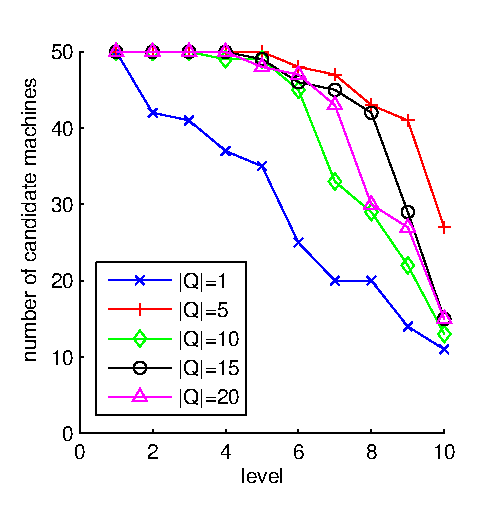
\includegraphics[scale=0.45]{Y3(b).eps}
}
\hspace{0.1cm}
\subfigure[Bandwidth consumption under different $|Q|$ and $m$] {
\label{fig:Y4(a)}
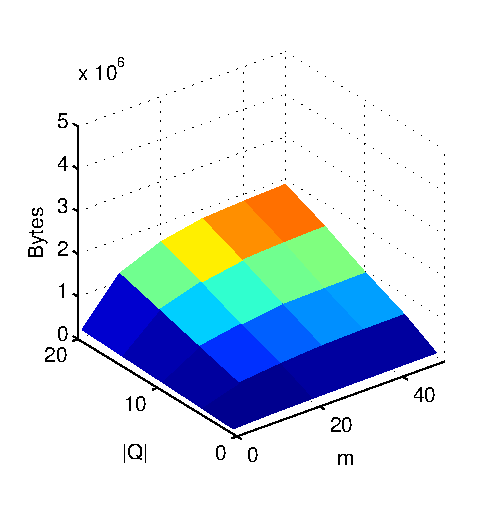
\includegraphics[scale=0.45]{Y4(a).eps}
}
\hspace{0.1cm}
\subfigure[Number of candidate machines in each level, $m$=50] {
\label{fig:Y4(b)}
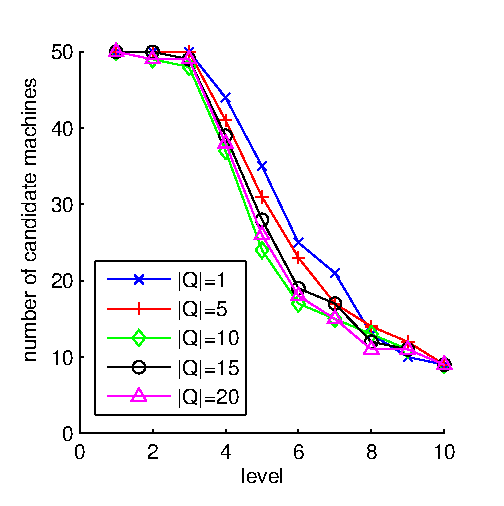
\includegraphics[scale=0.45]{Y4(b).eps}
}
\vspace{-0.05in}
\caption{Results of $k$NN queries using \MSWave-L{} with $d_{avg}$ for either
random reference sets ((a),(b)) or analogous reference sets ((c),(d)), 
$T$=1024, $k$=10}
\label{fig:Y3Y4}
\vspace{-0.1in}
\end{figure*}

\subsection{Sensitivity Analysis of \MSWave-L{} on Real Data}

The previous results have shown that \MSWave-L{} outperforms the other
frameworks.  To gain additional insights into its performance, we present
a further sensitivity analysis for \MSWave-L{} in this section.
%We discuss how the bandwidth usage
%of \MSWave-L{} would be influenced by variables such as the size of the reference set, the type of reference set, and the distance measurements.

\begin{figure*}[tb]
\centering
\subfigure[$d_{avg}$] {
\label{fig:Y5(a)}
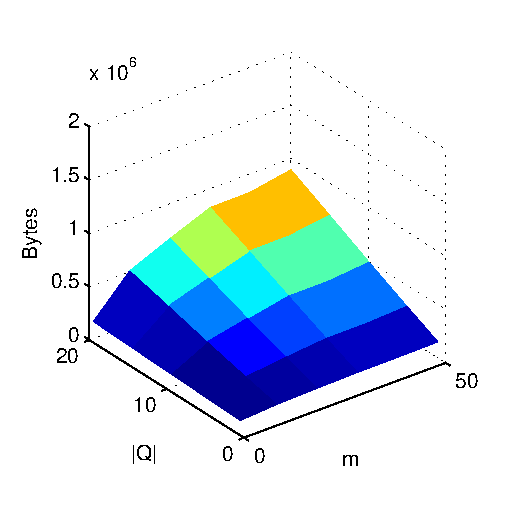
\includegraphics[scale=0.5]{Y5(a).eps}
}
\hspace{0.1cm}
\subfigure[$d_{sin}$] {
\label{fig:Y5(b)}
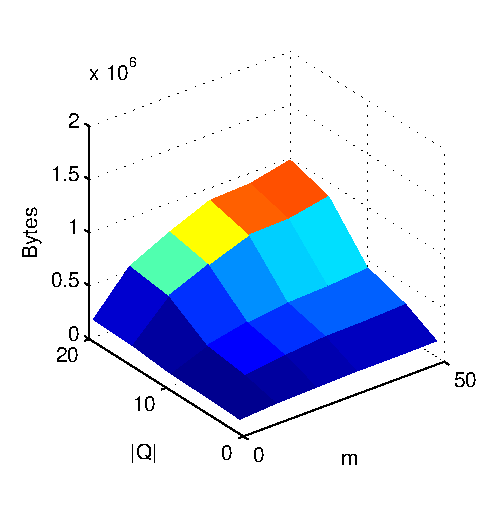
\includegraphics[scale=0.5]{Y5(b).eps}
}
\hspace{0.1cm}
\subfigure[$d_{com}$] {
\label{fig:Y5(c)}
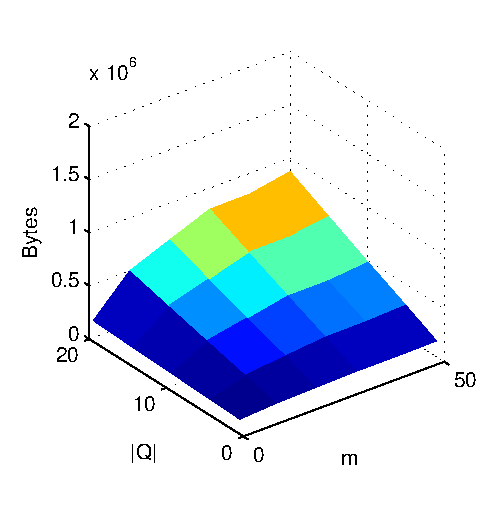
\includegraphics[scale=0.5]{Y5(c).eps}
}
\vspace{-0.05in}
\caption{Results for $k$FN queries with different linkage distances given analogous reference sets, $T$=1024, $k$=10}
\label{fig:Y5}
\end{figure*}

\textbf{Sensitivity to query set size and number of machines.}  First,
we examine the impact of the size of the reference set $|Q|$ and the
number of machines $m$ on the bandwidth consumption for finding $k$NN
under $d_{avg}$. In this experiment, we fix $k$=10 and $T$=1024, while
$|Q|$ is varied from 1 to 20 and $m$ is varied from 1 to 50, and we
consider both the random and analogous reference sets.
Figs.~\ref{fig:Y3(a)} (random) and \ref{fig:Y4(a)} (analogous) show
that the bandwidth consumption generally increases as $|Q|$ increases. 
An exception occurs for the random reference sets, where the bandwidth 
consumption of $|Q|$ = 10 is smaller than $|Q|$=5. By looking into
Fig.~\ref{fig:Y3(b)} we find that the pruning power of $|Q|$=10 was
also better than that of $|Q|=5$. This is because when the size of
the reference set increases from $|Q|$=5 to $|Q|$=10, certain reference
time series that are close to many candidates were included in the set,
which enables \MSWave-L{} to quickly prune many candidates. A similar
effect can be seen in Fig.~\ref{fig:Y4(b)} for the analogous reference
sets. In this case, the bandwidth consumption of \MSWave-L{} does not
increase too much with the growth of $|Q|$, which matches our
discussion in the previous section.

\textbf{Sensitivity to distance measure.} 
Finally, we examine the influence of the different distance
measures. We compare the three distance measures using analogous
reference sets to do $k$FN queries when $T$=1024, $k=10$, $|Q|$ is
varied from 1 to 20 and $m$ is varied from 1 to 50. As shown in
Fig.~\ref{fig:Y5}, we can see little difference between the measures
in terms of bandwidth consumption. The reason is that when the patterns in the
reference set are very similar to each other, the distances between
an arbitrary candidate series and each reference series is very
close. Thus, their $d_{avg}$, $d_{sin}$, and $d_{com}$ should be
similar. As a result, the bounds obtained in every round are similar,
and so are the final results. On the other hand, for random reference
sets, we find no consistent patterns among the three distance
measures. The bandwidth consumption indeed depends on how the reference
set is chosen.


\subsection{Comparison on Large-scale Synthetic Data}

We conclude our experimental study with a comparison of the five
frameworks on the large-scale synthetic data set discussed in
Section~\ref{subsec:setup}.  The purpose is to compare their bandwidth
consumption when the number of time series and the length of each time
series are much larger, namely, both are increased to 12,500.  Recall
that both \MSWave{} and \LeeWave-M{} can work when the time series
pattern length is not a power of 2. We also increase the total number
of machines to 500.

Fig.~\ref{fig:11(a)} shows the bandwidth consumption of all frameworks
using a logarithmic scale under the parameter settings $T=$12,500,
$k=30$, $m=500$, $d_{com}$, $k$FN, and the random reference set,
varying $|Q|$ from 10 to 50. The bandwidth savings for \MSWave-L{} and 
\MSWave-S{} are even more dramatic, about 1 to 2 orders of magnitude,
compared to CP, PRP, and \LeeWave-M{}. \MSWave{}'s advantage is fairly
consistent across the range of $|Q|$.  In addition, we also
observe the gap between \MSWave-L{} and \MSWave-S{} increases as
$|Q|$ increases, again agreeing with the analysis in Eq.~\eqref{eq:bandwidthsaved}.

Finally, Fig.~\ref{fig:11(b)} focuses in on \MSWave-L{}, the best
framework, and shows the effectiveness of its candidate pruning at
each level for the large-scale data set. The parameter settings are
the same as the prior experiment. The significant drop in the number
of candidate machines when only the coefficients of the top-half
levels are passed is the main reason for its significant bandwidth
savings. The results in this section demonstrate the added advantage of
\MSWave-L{} when $m$ is large and much greater than $k$.

\begin{figure}[tb]
\centering
\subfigure[Bandwidth consumption of all frameworks] {
\label{fig:11(a)}
%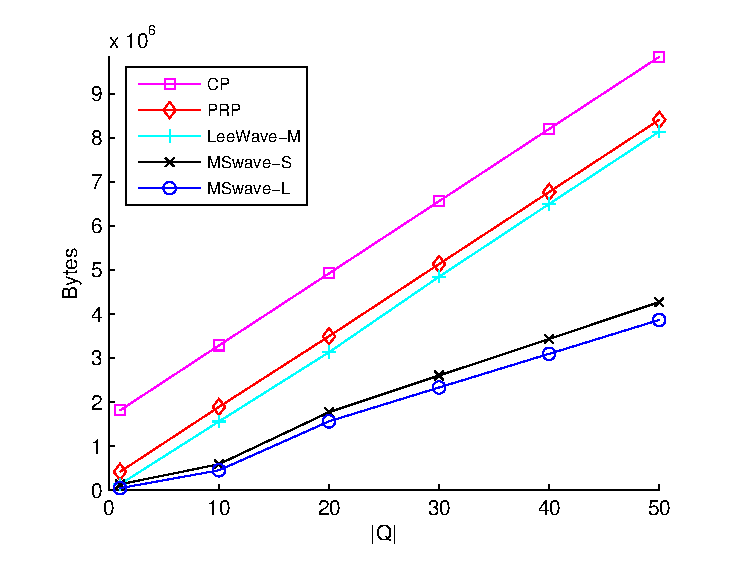
\includegraphics[scale=0.3]{1(a).eps}
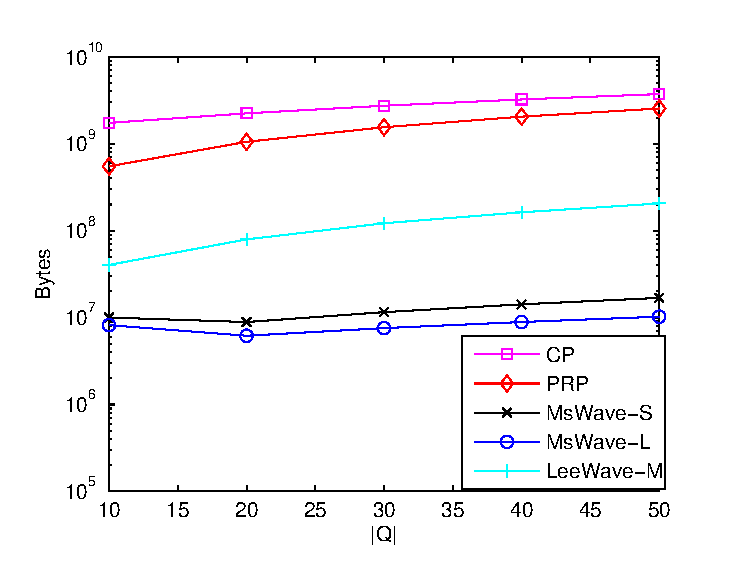
\includegraphics[scale=0.5]{5compare_log.eps}
}
\subfigure[Number of candidate machines in each level of \MSWave-L{}.] {
\label{fig:11(b)}
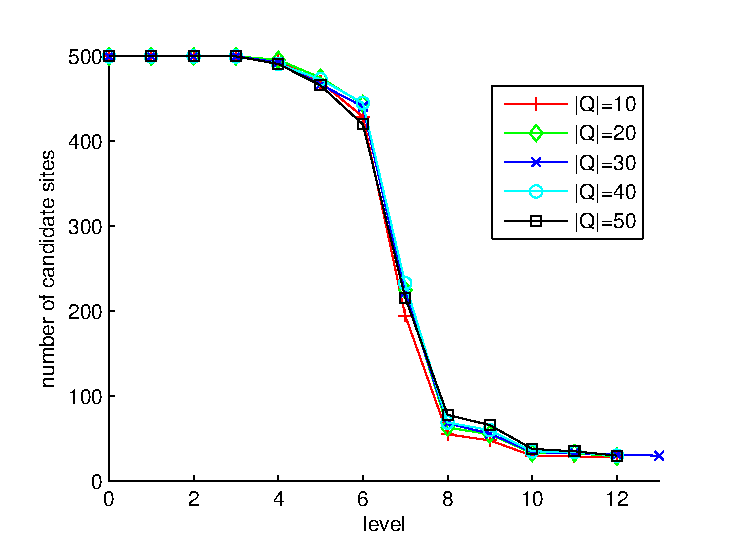
\includegraphics[scale=0.5]{rand_site_v2.eps}
}
\vspace{-0.05in}
\caption{\label{fig:11}
Experiments on synthetic data with random reference set, $T$=12500, $k$=30, $m$=500, $d_{com}$, $k$FN.}
\vspace{-0.05in}
\end{figure}



\section{Related Work}

Similarity search in time series databases has drawn wide attention
in recent years, due to its importance in many applications.
In particular, $k$-nearest neighbor search is a well-studied topic in both
fixed and streaming time series environments, such as the work
in~\cite{KOU04APP,LIU03EFF,HUN06EFF,Kashyap:2011:SKS}. 
% Gao et al.~\cite{GAO02EVA} proposed to continuously retrieve the latest
% $L$ points of a stream as a query pattern to find the nearest
% neighbors from a time series database via some prefetching
% technique. 
Given an error bound, Koudas \etal~\cite{KOU04APP}
approximated $k$-nearest neighbors search among stream snapshots. Liu
\etal~\cite{LIU03EFF} proposed a new indexing technique based on
scalar quantization to provide efficient nearest-neighbor search among
multiple streams. Hung and Chen~\cite{HUN06EFF} provided an efficient
approach to finding the $k$-nearest neighbors under an arbitrary range
constraint based on the Haar wavelet synopses. Kashyap \etal~\cite{Kashyap:2011:SKS} 
proposed a scalable $k$NN search method
for vertically stored time series. Based on a multi-resolution
transform on time series, the $k$NN search can be done by
progressively pruning candidates efficiently in a stepwise
sequential-scan manner. With different indexing and approximation
methods, the general goal is to get the $k$NN as efficiently as possible
from a large number of candidate time series.  All these works assume that
streams are collected and processed at a central site.

There are a number of works studying issues for time series stored in a
distributed environment, such as aggregation queries, burst detection,
and frequent pattern mining while
preserving privacy~\cite{Rastogi:2010:DPA,Singh:privacy,daSilva:2007:PPP}. However,
only a few works discuss similarity search or nearest neighbor search
for distributed time series. For example, Papadopolous and Manolopoulos~\cite{PAP01DPS}
analyzed four schemes to tackle $k$NN queries, and our earlier work
proposed \LeeWave{}~\cite{Yeh:2008:LLD}.
Both studies considered only single time series as the reference for queries
and did not address the $k$FN query problem.

Other work has studied queries containing multiple instances, but in
different settings. For example, in
multiple pattern matching in text search or bioinformatics 
applications~\cite{Kandhan:2010:SFS,Kim99afast}, the inputs are
assumed to be multiple strings and the algorithms report all
occurrences of the input strings. This is different from our goal of
finding $k$NN/$k$FN in continuous time series while limiting
bandwidth consumption. Meanwhile, the typical assumption of centralization
in these settings aims to speed up the processing, in contrast to our setting
where data are assumed to be coming from distributed sources. Furthermore, our
unified framework allows us to handle both similarity and
dissimilarity matching, which have been treated as two independent
problems in most of the previous works.

To the best of our knowledge, this paper is the first to deal with both $k$NN
and $k$FN queries for a reference set of multiple time series in a
distributed environment.

%Handling queries that contains multiple instances has attracted certain level of attention in the past years. For example, the multiple pattern matching for string in text search or bioinformatics~\cite{Kandhan:2010:SFS,Kim99afast} and exemplar-based recognition and learning~\cite{}. For multiple pattern matching, the inputs are assumed to be multiple strings and the algorithms tried to report all occurrences of them efficiently. It is different from our goal in finding $k$NN/$k$FN in continuous time sequence while using small bandwidth. Furthermore, the assumption of penalization aims at speed up the process, rather as our case to assume data are coming from distributed sources. For exemplar-based learning, they assumes all patterns are similar to some extent to perform learning, while in our framework such assumption is relaxed and we consider a more challenging setup as distributed sources. Furthermore, our unified framework allows us to handle both similarity and disilarity matching all together, which have been treated as two independent problems in most of the previous works. 

\section{Conclusions and Future Work}
\label{sec:conclusion}
\balance

%Many believe distributed computation will become inevitable in big data era not just because we need to speed up the processing but also due to the fact that data are likely to be stored distributedly. Time series data are of no difference as they are generating in a very fast speed, usually from sensors in a Machine-to-Machine environment. As have been reported by McKinsey in a white paper about big data, a Boeing 737 generates 240 terabytes of data during a single cross-country flight. Such huge amount of time series data have to be stored in a distributed database. To efficiently handle ad hoc queries to the database, or to even design a search engine in such a distributed environment that to concurrently process large amount of complex queries while still guarantee the quality of the results without consuming too much bandwidth and transmission cost, \MSWave{} seems to be a reasonable framework to be considered.


Distributed computation is generally believed to be a reasonable and
inevitable solution for M2M applications. It is not only because
huge amounts of data such as sensor readings are being accumulated fast and
distributedly, but also because of concerns of communication efficiency among
thousands or more devices. \MSWave{} provides the first framework for
efficiently and correctly handling ad hoc $k$NN/$k$FN queries with multiple
reference patterns over distributed time series data.

%in M2M systems, or even to design a search engine in such a
%distributed environment capable of concurrently processing large
%time series queries, while still guarantee the quality of the
%results, \MSWave{} seems to be a reasonable framework to be
%considered.

Technically speaking, compared with centralized nearest neighbor
search for time series, distributed time-series matching has been
studied by only a few prior works, none of which considered more
complex query patterns such as multiple time series. Although this
paper advances the state-of-the-art by introducing the multiple-series
query, we believe there are still many unresolved issues to be explored.
For example, we would like to investigate
how to improve the response time of such queries, which is constrained by
the current one-level-at-a-time approach; 
% instead of sending coefficients one level at a time, how to design a more flexible
% mechanism to transmit them considering different communication constraints; 
how to extend the proposed distributed time series matching
mechanism to supervised/semi-supervised learning in a distributed environment; 
how to extend \MSWave{} to other types of distance measures such as dynamic time warping; 
and how to resolve other types of complex queries such as ``find instances similar to at 
least $k$ reference instances.''  These and other open questions make for promising
directions for future work.



%
% The following two commands are all you need in the
% initial runs of your .tex file to
% produce the bibliography for the citations in your paper.
\bibliographystyle{abbrv}
\bibliography{miyen}  % sigproc.bib is the name of the Bibliography in this case
% You must have a proper ".bib" file
%  and remember to run:
% latex bibtex latex latex
% to resolve all references
%
% ACM needs 'a single self-contained file'!
%
%\input{appendix}
\end{document}
